\chapter{Denser Environments Cultivate Larger Galaxies: A Comprehensive Study Beyond the Local Universe with Hyper Suprime-Cam} \label{chap:morph_den}

{\large \emph{Aritra Ghosh, C. Megan Urry, Meredith C. Powell, Rhythm Shimakawa, Daisuke Nagai}} 


The relationship between galaxy size and environment has remained enigmatic, with over a decade of conflicting results. %and a lack of consensus. 
We present one of the first comprehensive studies of the variation of galaxy radius with environment and conclusively demonstrate that past conflicting results have been largely the result of small sample sizes and lack of robust measurement uncertainties. We correlate projected two-dimensional densities over $\sim360$ deg$^2$ with the structural parameters of $\sim3$ million Hyper Suprime-Cam galaxies at $0.3 \leq z < 0.7$ with $\log M/M_{\odot} \geq 8.9$. Compared to most previous studies, this sample is $\sim100-10,000$ times larger and goes down $\sim1$ dex deeper in mass completeness. We confirm with $>5\sigma$ confidence that galaxies in denser environments are $\sim10-20\%$ larger than equally massive counterparts in less dense regions of the Universe. We verify the presence of the above correlation individually in disk-dominated, bulge-dominated, star-forming, and quiescent sub-populations. We find the strength of the correlation to be dependent on redshift, stellar mass, and galaxy morphology. The correlation is strongest at lower redshifts and systematically weakens/disappears beyond $z \geq 0.5$. At $z\geq0.5$, massive bulge-dominated/quiescent systems and galaxies with $\log M/M_{\odot} \geq 11.25$ still display a statistically significant correlation. We posit that the above correlations are primarily driven by assembly bias in dark matter halos and the prevalence of galaxy mergers in denser environments. We also use the above sample to revisit the correlation between morphology and environment.  
%Consistent with previous results, we find that the fraction of bulge-dominated galaxies increases in denser environments.


\section{Introduction} \label{sec_c4:intro}

The morphological features and structural parameters of galaxies serve as a cornerstone in comprehending their attributes and have played an instrumental role in our understanding of galaxy formation and evolution. Since the dawn of the mid-20$^{th}$ century, astronomers have studied the intricate correlations between morphology and other fundamental properties of galaxies, leveraging these relationships as powerful tools to further our understanding of galaxy evolution.

Some early pioneering studies, such as \citet{holmberg_58}, unveiled a correlation between the morphology of galaxies and their stellar populations. They found that massive elliptical galaxies typically house older stars and exhibit limited star formation. In contrast, spiral galaxies mostly harbor younger stars and are actively engaged in star formation. This observed correlation has been used to suggest that early-type galaxies may halt star formation due to gas scarcity, possibly caused by  stellar or AGN feedback, or environmental effects. Conversely, late-type galaxies' ongoing star formation may stem from their ability to keep or acquire gas, potentially due to their lower masses or more isolated settings. We refer the interested reader to \citet{morph_review} for a detailed review.

Another early insight observed was the relationship between a galaxy's morphology and its environment. \citet{dressler_84} found that elliptical galaxies are more common in high-density regions of the universe, such as the centers of galaxy clusters; while spiral galaxies are more common in low-density regions, like the outskirts of clusters or in the field. This observation was one of the first suggestions of a strong link between a galaxy's environment and its evolution --- a concept that remains an active area of research even to this day.  

Since then, subsequent studies have substantiated this relationship, and there is now considerable evidence showing that whether a galaxy is elliptical or spiral depends to a large degree on the density of that particular galaxy's environment \citep[e.g.,][]{gomez_03, vdw08, blanton_09, Tasca09, Cappelari11, Fogarty14, hsc_morph_den}. Although the evidence gets more sparse at higher redshifts, the effect has also been shown to exist in the high redshift universe till $z\sim2-3$. We should note that some studies suggest that this trend nearly vanishes at a fixed stellar mass, implying that mass could be the predominant factor controlling this observational trend \citep[e.g.,][]{Holden07, Bamford09, Brough17, Greene17}.

\begin{table}[htbp]
    \small
    \centering
    \caption{Previous Observational Studies of Environmental Dependence of $R_e$ at $z \geq 0.2$\label{tab_c4:lit_survey}}
    \begin{tabular}{P{2cm}P{2cm}P{1.4cm}P{1.5cm}P{1.5cm}P{1.25cm}P{2.3cm}}
    \hline
    \hline
    Reference & Survey / Instrument\textsuperscript{a} & Redshift  & Stellar Mass ($\log M / M_{\odot}$) & Sample Size & Density Measure\textsuperscript{b} & Radius - Env. Correlation\textsuperscript{c}\\
    \hline
    \hline
   \citet{Siudek22} & VIPERS & $0.5 - 0.9$ & $9 - 11.5$ & $\sim 30,000$ & Density Contrast & $+$ve \textit{only} for blue galaxies \\
    \hline
    \citet{Gu21} & CANDELS & 0.5 - 2.5 & $\geq 9.2$ & $\sim13,500$ & Density Contrast & No correlation \\
    \hline
    \citet{Afonso19} & VIMOS & 0.8 - 0.9 & $\geq 10$ & $\sim 500$ & Density Contrast & $+$ve \textit{only} for galaxies with $\log M/M_{\odot} > 11$ \\
    \hline
    \citet{Matharu19} & HST & $\sim1$ & $\geq10$ & $\sim600$ & Cluster/ Field & $-$ve correlation \\
    \hline
    \citet{Chan18} & KMOS/HST (passive only) & 1.39 - 1.61 & $\geq10.2$ & $\sim3000$& Cluster/ Field & $+$ve in two clusters; $-$ve in one\\
    \hline
    \citet{Kelkar15} & ESO Distant Cluster Survey & 0.4 - 0.8 & $\geq 10.2$ & $\sim400$ & Cluster/ Field & No correlation\\
    \hline
    \citet{Allen15} & ZFOURGE/ CANDELS & $\sim2.1$ & $\geq 9$ & $\sim500$ & Cluster/ Field & $+$ve \textit{only} for star-forming galaxies\\ 
    \hline
    \citet{Bassett13} & CANDELS & $\sim1.6$ & $ \geq 10.3$ & $\sim 500$ & Cluster/ Field & $+$ve \textit{only} for quiescent galaxies\\
    \hline
    \citet{Huertas-Company13}  &  COSMOS (passive only) & 0.2 - 1.0 & $\geq 10.5$ & $\sim700$ & Cluster/ Field & No correlation for passive galaxies\\
    \hline
    \citet{Lani13} & UKIDSS & 1.0 - 2.0 & $\geq 10.4$ & $\sim96,000$ & Density Contrast & $+$ve \textit{only} for passive galaxies\\
    \hline
    \citet{Cooper12} & DEEP2/3 (passive only) & 0.4 - 1.2 & 10 - 11 & $\sim600$ & Density Contrast & $+$ve for passive galaxies\\
    \hline
    \hline
    \multicolumn{7}{p{0.95\textwidth}}{\vskip 0.01cm \small \textsuperscript{a} Note that some studies only included passive galaxies in their sample and have been denoted accordingly.} \\
    \multicolumn{7}{p{0.95\textwidth}}{\small \textsuperscript{b} ``Density Contrast" refers to a numerical measurement of overdensity either using the number of neighbors within a certain volume or distance to the $n^{th}$ nearest neighbor. ``Cluster/Field" refers to categorically separating galaxies into cluster and field galaxies, without any numerical measurement of overdensity.} \\
    \multicolumn{7}{p{0.95\textwidth}}{\small \textsuperscript{c} $+$ve correlation refers to larger galaxies being present in denser environments. Note that for some of the rows, $+$ve correlation is noted as being observed for \textit{only} certain sub-populations --- this means that the authors investigated other sub-populations but did not find evidence for correlation.}
    \end{tabular}
\end{table}

In stark contrast to the relatively well-established morphology-environment correlation is the relationship between galaxy size (half-light radius; $R_e$) and environment. Despite having been studied for more than a decade, this relationship remains enigmatic, with no broad consensus in the field. Beyond the local universe ($z \geq 0.2$), different studies have reported wildly conflicting results, as summarized in Table \ref{tab_c4:lit_survey}. While some studies have reported a positive correlation of radius with the environment for certain sub-populations of galaxies \citep[e.g.,][]{Cooper12,Lani13,Bassett13,Afonso19,Siudek22}; some studies have reported no correlation \citep[e.g.,][]{Huertas-Company13, Kelkar15,Gu21}; and some have reported negative correlation \citep[e.g.,][]{Matharu19,Chan18}. Although not a focus of this study, the said disagreement also extends to the local universe \citep[e.g.,][]{Blanton05, Park07, Cappellari13, Huertas-Company13_local, Yoon17}. These above observational results are even more surprising given that hierarchical models of galaxy formation in the $\Lambda$ cold dark matter ($\Lambda$CDM) paradigm have consistently predicted galaxy sizes to be linked to the properties of their dark matter halos and their environment \citep[e.g.,][]{shankar13, Kravtsov13, somerville18, jiang19}. We will discuss later in \S \ref{sec_c4:theory} how our new results broadly agree with these theoretical frameworks. 

The conflicting results discussed above can primarily be attributed to several challenges faced in previous studies. These include:- a) the absence of statistically significant sample sizes; b) the presence of systematic discrepancies between measurements obtained from different surveys employed in the same study (e.g., between cluster and field galaxies); c) the absence of robust uncertainty estimates on the measurements of galaxy radius; d) not using statistically robust frameworks to assess the presence of correlations. 

The limited sample sizes used in prior studies are particularly problematic due to their inability to account for:- i) the great diversity in the nature of dense environments (e.g., different galaxy clusters); ii) rare objects (e.g., massive galaxies) which might play an important role in controlling the environmental dependence. Additionally, given that galaxy sizes are primarily dictated by galaxy mass, any correlations with environment will be secondary/weaker; and necessitates a careful, statistically robust analysis. Therefore, having robust estimates of uncertainties on $R_e$ measurements and accounting for them in the correlation analysis is extremely important.  

Clearly, one needs large uniform samples of galaxies with excellent imaging quality coupled with robust statistical frameworks to accurately measure galaxy sizes and examine their correlation with environment over a broad range of stellar mass and redshift. The excellent imaging quality of the Hyper Suprime-Cam Subaru Strategic Program (HSC-SSP), in conjunction with state-of-the-art Bayesian machine learning (ML) frameworks like the Galaxy Morphology Posterior Estimation Network (\gampen{}), offers an unprecedented opportunity and puts us in a unique position. 

For the first time, we simultaneously have access to radius measurements with accurate uncertainties for millions of galaxies beyond the local universe, as well as measurements of environmental density covering $\sim360$ deg$^2$. Using this, in this article, we present the  first comprehensive study of the variation of galaxy radius with environment beyond the local universe. We also briefly revisit the variation of galaxy morphology with environment using our comprehensive sample. While most previous studies of morphology v/s environment used qualitative classification schemes to discern morphological types, we use the quantitative measure of bulge-to-total light ratio ($L_B/L_T$) to separate different morphological types. 

The robustness of \gampen{} coupled with the depth of the HSC data enables us to assemble a large uniform sample of $\sim3$ million galaxies in the redshift range $0.3 \leq z < 0.7$ down to $\sim23$ AB mag. This sample size is $\sim100-10,000$ times larger than most previous studies and is mass complete to $\sim1$ dex more than most previous studies. Using the full Bayesian posteriors predicted by \gampen{} combined with a Monte-Carlo analysis framework, we are able to incorporate the uncertainties in $R_e$ measurements into our correlation analysis. This allows us to confirm/reject the presence of correlations with very high statistical significance --- in most cases with $>5\sigma$ confidence.

We use the comprehensive galaxy morphology catalog for HSC galaxies that was obtained using \gampen{} (see Chapter \ref{chap:hsc_morph}); and correlate these structural parameter measurements with the wide-field projected density map available from HSC-SSP \citep{hsc_den}. We study the variation of both effective radius as well as morphological fractions on a 10 co-moving Mpc ($10\,\,cMpc$) scale ---  thus focusing on the large-scale environmental effect by taking advantage of the wide-field coverage of HSC ($\sim 360$ deg$^2$). We investigate the above correlations for the overall sample of galaxies as well as for four sub-populations of galaxies derived from the main sample -- disk-dominated, bulge-dominated, star-forming, and quiescent galaxies.

In \S \ref{sec_c4:data}, we describe our sample selection as well as the determination of structural parameters, density, mass, and separation of galaxies into the various sub-populations. \S \ref{sec_c4:results} outlines the results of the above-mentioned correlation analysis for both $R_e$ and disk-/bulge-dominated morphological fractions. We summarize our findings in \S \ref{sec_c4:discussion} and outline the theoretical framework that can be used to understand our results. We end with the primary takeaways of this study as well as future directions in \S \ref{sec_c4:conclusions}. Throughout this work, we use AB magnitudes and Planck18 cosmology ($H_0=67.7$ km/s/Mpc, \citealp{planck18}).

\section{Data} \label{sec_c4:data}
We use data from the Hyper Suprime-Cam Subaru Strategic Program Public Data Release 2 \citep[PDR2;][]{hsc_pdr2}. Specifically, we use the Wide layer of PDR2, which covers $\sim360$ deg$^2$ in all five broad-band filters (\gb\rb\ib\zb\yb) and reaches a depth of $\sim26$ AB mag. In the next few subsections, we will outline our sample selection as well as the various external catalogs used for this study. 

\subsection{Sample Selection} \label{sec_c4:sample_selection}
The starting point for our sample selection is galaxies with $0.3 \leq z \leq 0.7$ from the morphological catalog produced in Chapter \ref{chap:hsc_morph}. The said catalog includes most HSC-Wide extended sources with $m < 23$. We only include sources with more than five sigma detection (in the \texttt{cmodel} measurement) in all HSC bands and exclude galaxies near bright stars or with significant imaging issues (e.g., cosmic ray hits, saturated pixels) identified using the \texttt{mask\_s18a\_bright\_objectcenter} and \texttt{cleanflags\_any} parameters in PDR2. 
%bring stars -- (mag $<17.5$)

For all galaxies in our sample, we use high-quality photometric redshifts from the second data release of the HSC photo-z catalog \citep{photoz_hsc_pdr2}. These redshifts were calculated from HSC five-band photometry by using Mizuki \citep{mizuki}, a Bayesian template fitting code, and we refer the interested reader to \citet{photoz_hsc_pdr2} for more details. For $m < 23$ HSC-Wide galaxies, the bi-weight dispersion of $\Delta z=\left(z_{\text {photo }}-z_{\text {spec }}\right) /\left(1+z_{\text {spec }}\right)$ is $\leq 0.05$. To further isolate a sub-sample with secure photometric redshifts, we only include galaxies for which the \texttt{photoz\_risk\_best} parameter $<0.1$. This parameter controls the risk of the photometric redshift being outside the range $z_{\mathrm{true}} \pm 0.15(1+z_{\mathrm{true}})$, with 0 being extremely safe to 1 being extremely risky. We also exclude galaxies with reduced chi-square $\chi_{\nu}^2 > 5$ for the best-fitting model, as recommended by \citet{photoz_hsc_pdr2}. Following \citet{hsc_den}, we employ a further selection cut for galaxies in $0.4 \leq z \leq 0.5$, where there is a strong Balmer-Lyman break degeneracy. To minimize potential contamination from Lyman break galaxies at $z\sim3$, we exclude galaxies that have specific star-formation rates (sSFRs)  $> 1$ Gyr$^{-1}$. This is because misclassified objects at $z\sim3$ mostly show very young ages ($\sim 1$ Gyr) with very high sSFRs. Note that the contamination of Lyman break galaxies for higher redshift bins, including \ib-band dropouts, is negligible given our detection criteria in all HSC bands, including the \gb-band. 

Thereafter, we split our sample into four different redshift slices:- $0.3 \leq z < 0.4$, $0.4 \leq z < 0.5$, $0.5 \leq z < 0.6$, and $0.6 \leq z < 0.7$. Within each redshift slice, we match the positions of galaxies in our sample to the fine-grid of HSC PDR2 survey locations at which density measurements are available from the \citet{hsc_den} catalog (see \S \ref{sec_c4:density_measurements} for more details). Based on the grid size used in \citet{hsc_den}, we allow for a maximum positional error of $64\arcsec$ and discard all unmatched sources. This step ensures that the two survey areas (of morphology and density estimation) are completely consistent with each other. Note that the \citet{hsc_den} catalog also included $m < 23$ sources with more than five sigma detection in all HSC bands and followed a data-cleaning procedure very similar to ours (see \S 2 of \citet{hsc_den}). This leaves us with a final sample of $\sim2.9$ million galaxies, with $0.49$ million, $0.70$ million, $0.65$ million, and $1.05$ million in the four redshift bins, respectively.   

\subsection{Morphology Measurements} \label{sec_c4:morph_measurements}
The bulge-to-total light ratio ($L_B/L_T$) and effective radius ($R_e$) measurements used in this work are from the morphological catalog in Chapter \ref{chap:hsc_morph} and were obtained using the Galaxy Morphology Posterior Estimation Network (\gampen{}; see Chapter \ref{ch:gampen}). \gampen{} is an ML framework that can estimate full Bayesian posteriors for different structural parameters of galaxies and has been extensively tested both on simulations and HSC-Wide data (see Chapters \ref{ch:gampen} \& \ref{chap:hsc_morph}). \gampen{}'s predicted posterior distributions are extremely well-calibrated ($\lesssim 5\%$ deviation) and outperform uncertainty estimates from light-profile fitting codes by $\sim15-60\%$ (see Figure \ref{fig_c3:cov_prob_comp_euclud}). Specifically for $R_e$ measurements of $0.3 \leq z <0.7$ HSC-Wide galaxies, the dispersion in \gampen{}'s prediction error $\Delta R_e=\left(R_{\text {pred.}}-R_{\text {true}}\right) /R_{\text {true}}$ is $\leq0.07$. \gampen{}'s $R_e$ estimates of these galaxies have also been tested against measurements obtained using GALFIT \citep{galfit}. \gampen{}'s measurements have been found to be consistent overall and outperform that of GALFIT for galaxies with $R_e \leq 2\arcsec$ ($\sim 12.6$ kpc at $z=0.5$) (see Figure \ref{fig_c3:gampen_v_galfit}).

\begin{figure}[htb]
    \centering
    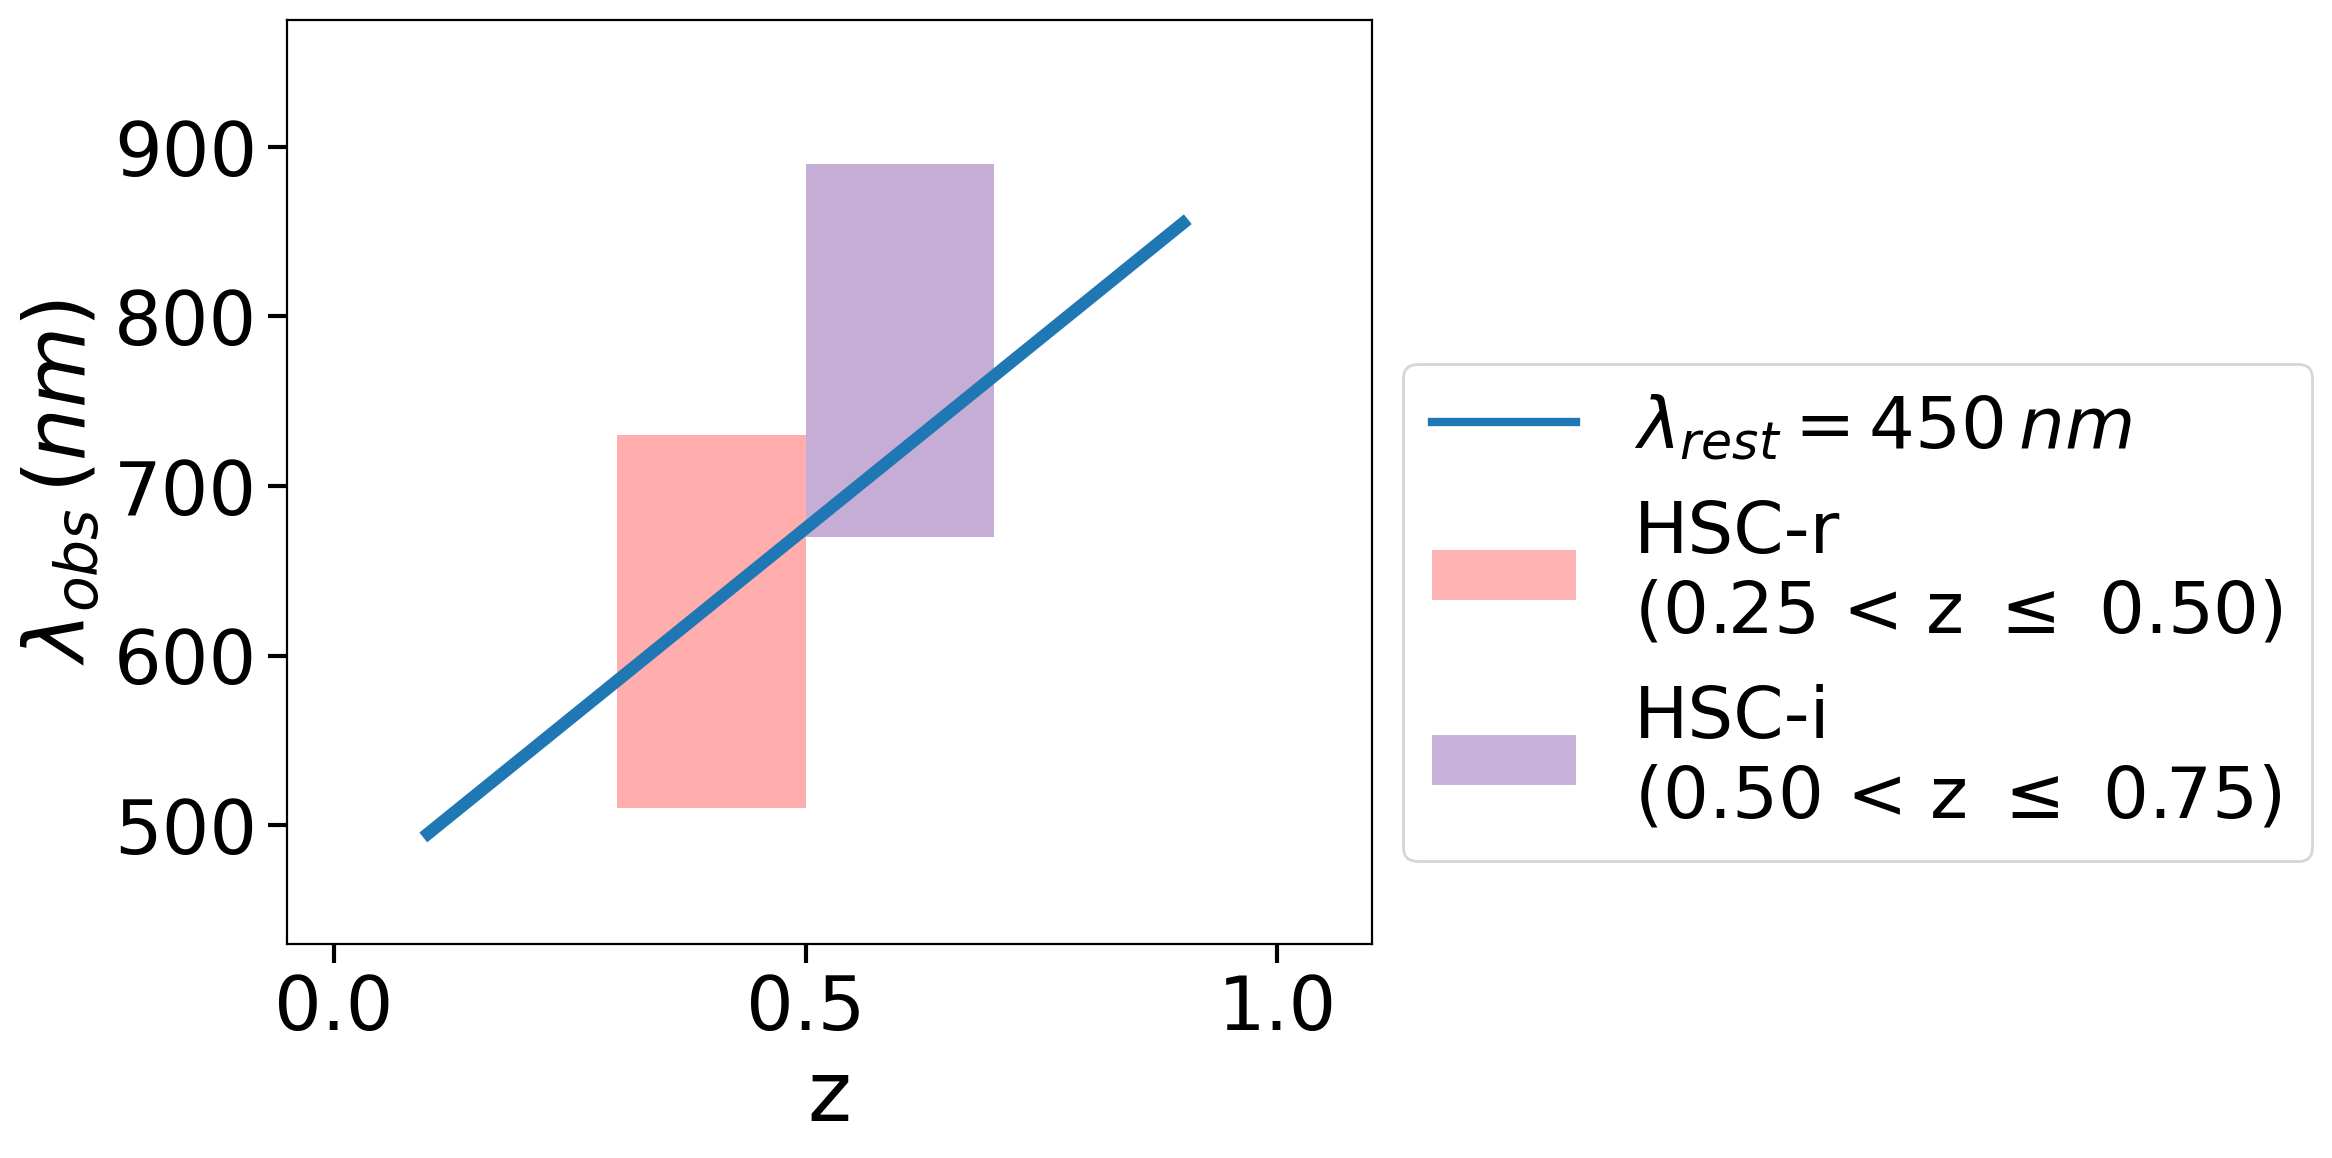
\includegraphics[width = 0.6\textwidth]{band_comp.png}
    \caption{The filter used for morphological determination for each redshift bin is shown along with the wavelength range sampled by each filter. The blue line shows where rest-frame $450\,\,nm$ emission falls for redshifts labeled on the x-axis. As this figure shows, the chosen filters allow us to consistently perform morphology determination at a rest-frame wavelength of $\sim450\,\,nm$ (i.e., in the rest-frame \gb{}-band).}
    \label{fig_c4:band_comp}
\end{figure}

As shown in Figure \ref{fig_c4:band_comp}, we use different imaging bands for galaxies at different redshifts --- this allows us to consistently perform morphology determination in the rest-frame \gb-band across our entire sample. We use \rb-band for $0.3 \leq z < 0.50$, and \ib-band for $0.50 \leq z < 0.7$. Additionally, as outlined in Appendix \ref{sec_c4:ap:size_corr}, we further investigated the effect of color gradients on our measured $R_e$ values by correcting them to a rest-frame wavelength of $450\,\,nm$. We found the applied size corrections to be $\lesssim5\%$, with no significant impact on the correlation coefficients reported in this study. 

For all structural parameters used in this study, we use the most probable value (mode) of the \gampen{}-predicted posterior distributions as the measured value and the width of the $68\%$ confidence interval as the error bar. Note that all measurements used in this study and the ML models used to obtain them are publicly available (see \S \ref{sec_c3:ap:data_access}).

\subsection{Density Measurements} \label{sec_c4:density_measurements}

The density measurements used in this study are from the \citet{hsc_den} catalog, which measured the projected two-dimensional density in five of the seven HSC-Wide fields, covering an area of $\sim 360$ deg$^2$. One of the five fields (\texttt{W04 GAMA12H}) is shown as an example in Figure \ref{fig_c4:hsc_den_map}. \citet{hsc_den} chose the $\sim 360$ deg$^2$ survey area by identifying regions in which the five sigma limiting magnitude of the point-spread function is deeper than $i=26$ -- this criterion was chosen to prevent the need for correction of the variance of number densities due to depth variation across the survey field. Note that both this study and \citet{hsc_den} use the same underlying catalog (HSC PDR2), and thus all catalog quantities (e.g., photometric redshifts) are consistent among the two studies.

\begin{figure*}[htb]
    \centering
    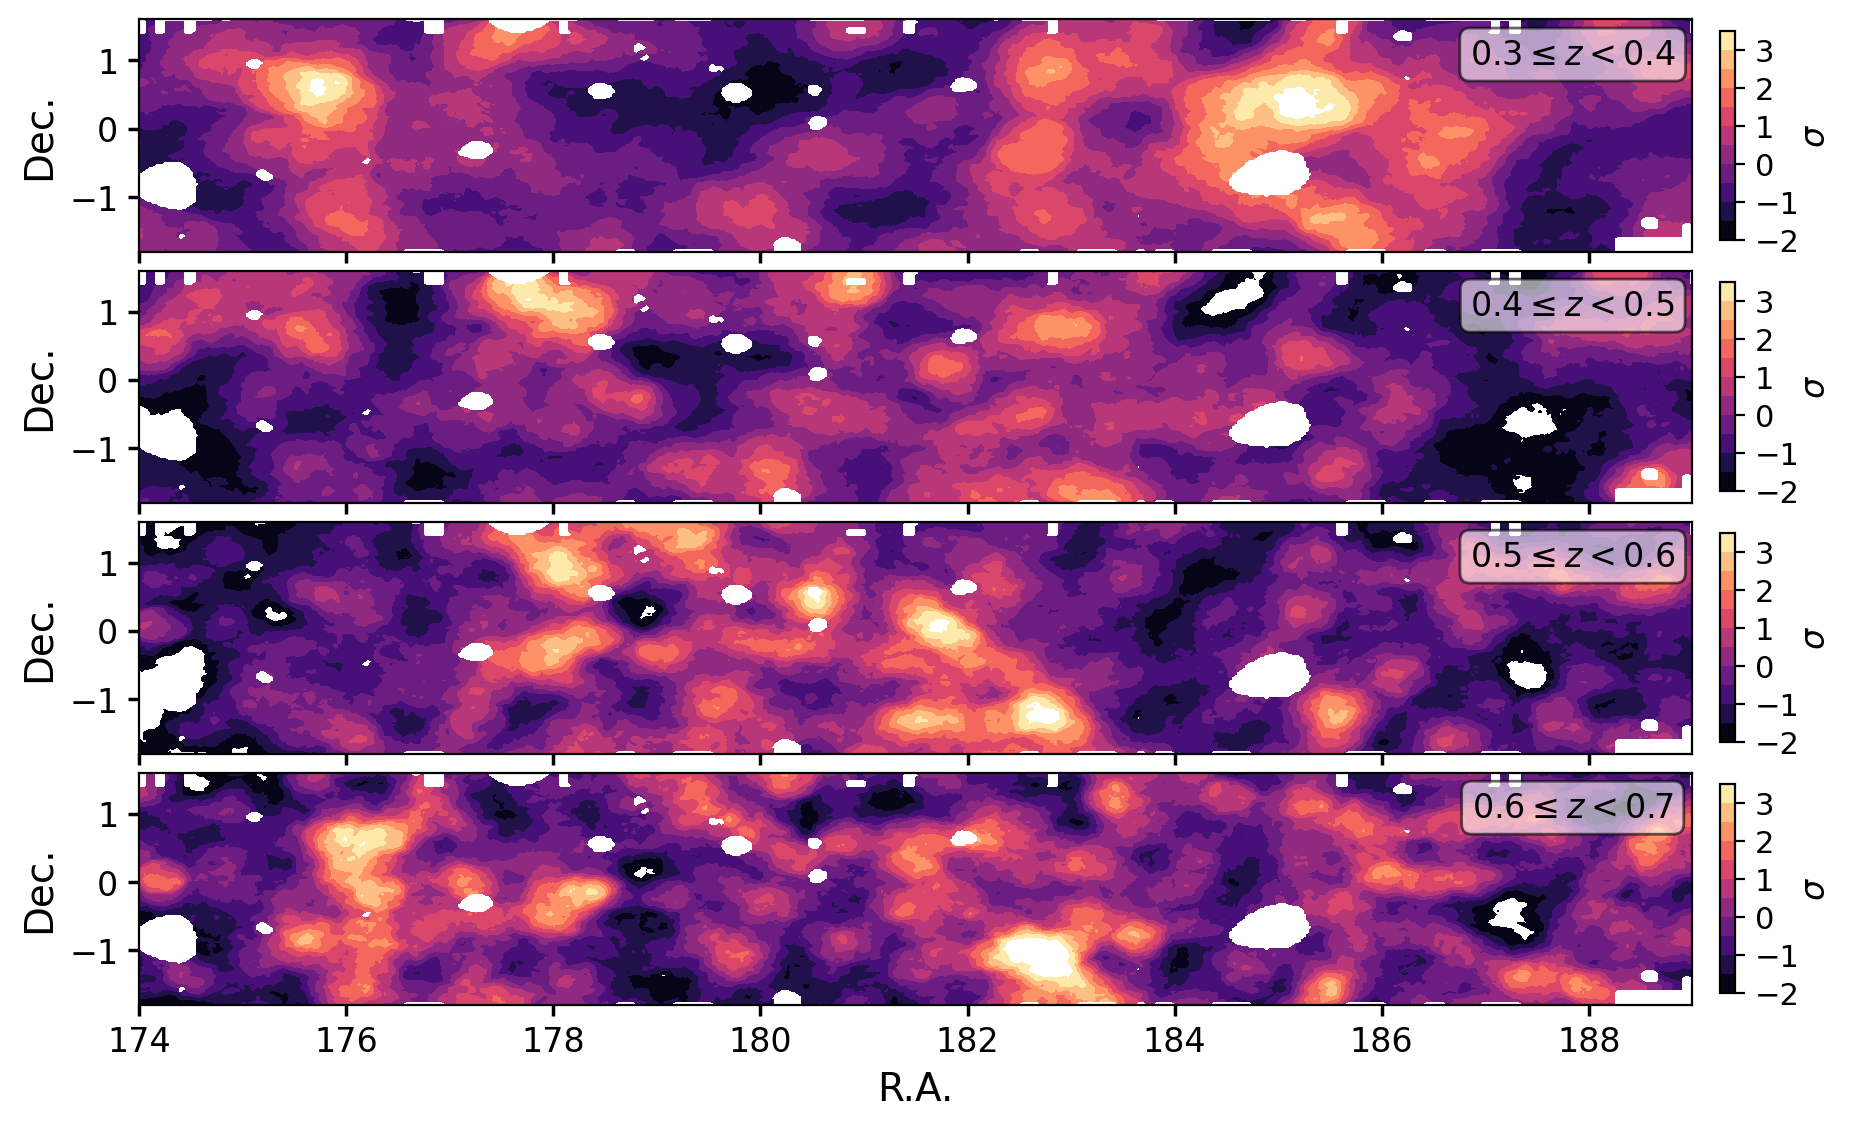
\includegraphics[width = \textwidth]{hsc_den_map.png}
    \caption{Projected two-dimensional densities are shown above for \texttt{W04 GAMA12H} --- one of the five HSC-Wide fields used in this study. Each row corresponds to a different redshift slice within which the densities are measured. Colors indicate the density excess in standard deviation within $r=10$ cMPc as denoted by the colorbars on the right. The white regions demarcate bright-star masks used during density measurement. Note that mask corrections are already incorporated into the density measurements used in this work, and we refer the interested reader to \citet{hsc_den} for more details.}
    \label{fig_c4:hsc_den_map}
\end{figure*} 

The projected density map has a spatial resolution of $\sim1.5\arcmin$, and the redshift slices constructed in this study mirror the ones used in \citet{hsc_den}. We set the density estimate at each grid point of the survey area to be the density excess measured using a top-hat aperture of $r=10$ co-moving Mpc ($\sigma_{r=10 cMpc}$) within the specific redshift slice. Note that \citet{hsc_den} tested their pipeline on a mock galaxy catalog and found that their projected over-densities well trace the total masses of embedded massive dark matter halos at each redshift slice. They also confirmed the consistency of their measurements at $z \leq 0.6$ against mean lens shear signals from a weak lensing stacking analysis. We refer the interested reader to \citet{hsc_den} for more details. 

\subsection{Stellar Masses} \label{sec_c4:mass_completeness}
The stellar masses used in this study are from the same Mizuki catalog that was used for photometric redshift estimates. We remind the reader that our study only includes sources with more than five sigma detection in all HSC bands, and we have also discarded sources with reduced chi-square $\chi_{\nu}^2 > 5$ for the best-fitting model. \citet{hsc_photoz_pdr1} and \citet{hsc_morph_den} have compared these stellar masses from Mizuki, based on HSC \gb{}\rb\ib\zb\yb{} photometry, against stellar masses obtained from the NEWFIRM Medium Band Survey \citep{newfirm} and COSMOS2015 \citep{cosmos_2015}; both of which are based on $>30$-band photometry. The above studies found the Mizuki measurements to be overestimates, especially at higher redshifts. However, at $z \leq 0.7$, this discrepancy is $\lesssim0.1$ dex. These differences can be attributed to the systematic differences in the data as well as the adopted template error functions and priors. Note that when comparing two independent surveys, stellar mass offsets of $\sim0.2-0.3$ dex can be expected even when both the data sets have deep photometry in multiple filters \citep[e.g.,][]{dokkum_14}.

\begin{figure}[htb]
    \centering
    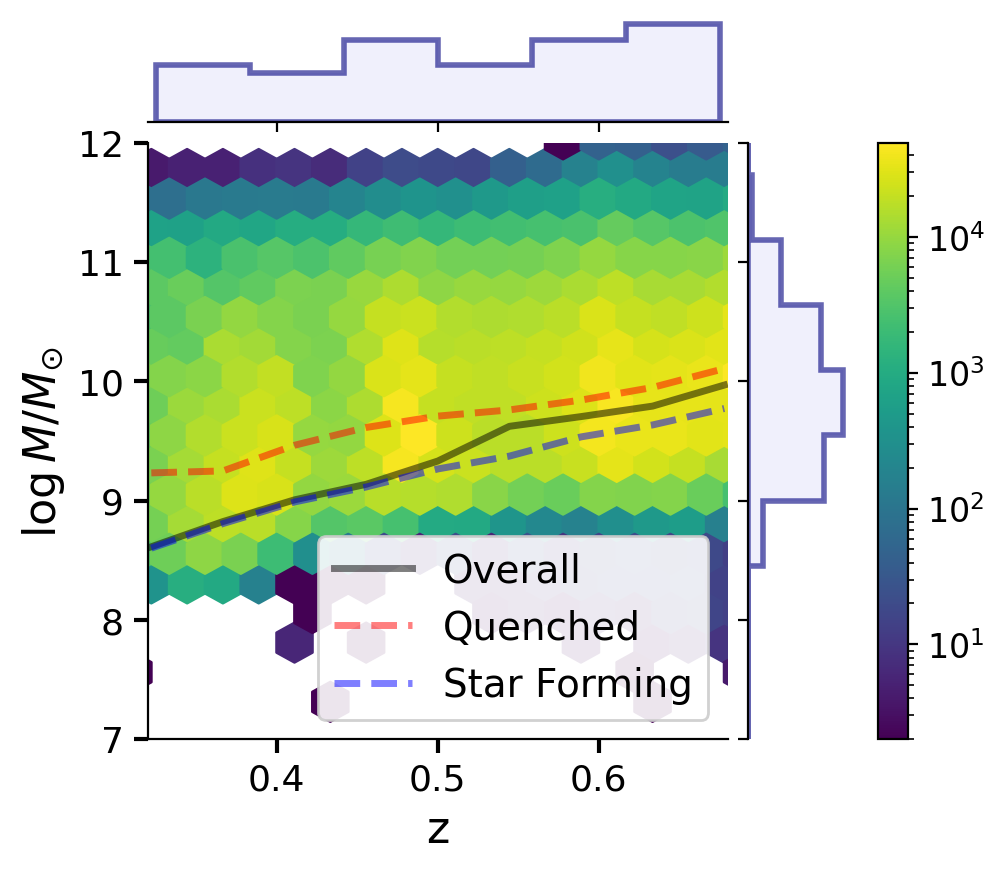
\includegraphics[width = 0.6\textwidth]{mass_comp_marg.png}
    \caption{The above figure shows the distribution of stellar mass as a function of redshift for all galaxies in our sample. The mass-redshift space is divided into hexagonal bins of roughly equal size, with the number of galaxies in each bin represented according to the colorbar on the right. Marginal histograms are also plotted along each axis. The solid black line shows the $90\%$ stellar mass completeness limit for the entire sample, while the red and blue solid lines show the mass completeness limits for the quiescent and star-forming sub-populations. The faint dotted lines demarcate each redshift slice's adopted lower mass limits ($M_c$).}
    \label{fig_c4:mass_comp}
\end{figure}

To estimate the $90\%$ stellar mass completeness limit of our sample, we follow the approach outlined in \citet{pozzetti_10} and \citet{Weigel16}. We select galaxies in narrow redshift bins and calculate their limiting stellar mass ($M_{lim}$) -- the mass they would have if their apparent magnitude were equal to $23$, the magnitude limit we chose for our sample. Thereafter, we selected $20\%$ of the faintest galaxies -- and defined the stellar mass completeness limit as the $90^{th}$ quantile  of $M_{lim}$ values in each redshift bin. Figure \ref{fig_c4:mass_comp} shows the determined mass completeness limit for all galaxies, as well as separate completeness limits for star-forming and quiescent galaxies (refer to \S \ref{sec_c4:sep_into_subsamples} for a description of how we isolate these sub-populations). Our sample is complete down to $\sim8.5 M_{\odot}$ at $z=0.3$ and $\sim10M_{\odot}$ at $z=0.7$. The completeness limits at the lowest and highest redshifts are 8.6$M_{\odot}$ (9.2$M_\odot$) and 9.9$M_\odot$ ($10.1 M_\odot$), respectively, for star-forming (quiescent) galaxies. To be conservative, we implement a step function on top of the obtained stellar mass completeness limit, as shown in Figure \ref{fig_c4:mass_comp}. The values of this step function are used as the lower mass limit ($M_c$) for each redshift slice and are shown in Table \ref{tab_c4:mass_comp}.

\begin{table}[htbp]
    \centering
    \caption{Lower Mass Limits ($M_c$) Used at Different Redshifts\label{tab_c4:mass_comp}}
    \begin{tabular}{c|ccc}
    \hline
    \hline
    Redshift Slice & \multicolumn{3}{c}{Lower Mass Limit ($\log M/M_\odot$)}\\
    & Overall & Quiescent & Star Forming \\
    \hline
    \hline
    $0.3 \leq z < 0.4$ & 8.95 & 9.41 & 8.91 \\
    $0.4 \leq z < 0.5$ & 9.33 & 9.66 & 9.23 \\
    $0.5 \leq z < 0.6$ & 9.72 & 9.90 & 9.55 \\
    $0.6 \leq z < 0.7$ & 10.09 & 10.15 & 9.87 \\
    \hline
    \hline
    \end{tabular}
\end{table}

\subsection{Separating Into Sub-Populations} \label{sec_c4:sep_into_subsamples}
In \S \ref{sec_c4:results}, we will explore the variation of structural parameters with environmental density for various sub-populations of galaxies derived from our main sample. To divide galaxies into disk- and bulge-dominated samples, we classify all galaxies with $L_B/L_T \leq 0.4$ as disk-dominated and all galaxies with $L_B/L_T \geq 0.6$ as bulge-dominated. 

To separate galaxies into star-forming and quiescent sub-samples, we use their rest-frame SDSS \uband{}-\rb{} v/s \rb{}-\zb{} colors, calculated using SED fitting. Use of the \uband{}-\rb{} v/s \rb{}-\zb{} color-color diagram has already been demonstrated to be an effective way to separate these sub-populations \citep[e.g.,][]{Holden12, Chang15, pozzetti_10, lopes_16, hsc_mass_size}. Note that for our sample, we are unable to use \textit{UVJ} selection because SED fitting using HSC \grizy{} photometry does not allow us to obtain robust estimates for rest-frame \textit{J} magnitudes. We obtain the SDSS rest-frame magnitudes from the same Mizuki catalog that was used for redshift and stellar mass estimation. 

\citet{hsc_mass_size} has demonstrated that applying the \citet{Holden12} \textit{urz} color-color selection directly to HSC data does not optimally distinguish quiescent and star-forming galaxies; instead, the boundaries need to be adjusted. Thus, we follow \citet{Kawin16} and \citet{hsc_mass_size} and use our sample to self-calibrate the region separating quiescent from star-forming galaxies. The final separation boundaries obtained and an extended description of the procedure are available in Appendix \ref{sec_c4:ap:cc_sel}.

\section{Results} \label{sec_c4:results}
The central focus of this work is to study how the structural parameters of galaxies vary as a function of their environmental density. In \S \ref{sec_c4:data}, we already described how a measurement of environmental density is assigned to galaxies from the Chapter \ref{chap:hsc_morph} morphological catalog. We now use this combined information to study how environment affects galaxy radius (\S \ref{sec_c4:rad_den}); and how the measured fractions of different morphological classes change as a function of environment (\S \ref{sec_c4:morph_env}).

\subsection{Variation of Radius with Environment} \label{sec_c4:rad_den}
We separate the galaxies in each redshift slice into five bins based on their environmental density. The bins are linearly spaced and span the range $\sigma_{r=10cMpc} = [-2,3)$. Thereafter, we investigate the distribution of half-light radius ($R_e$) within each bin. In \S \ref{sec_c4:rad_den_all}, we will outline our results for all galaxies in our sample. In \S \ref{sec_c4:rad_den_sub}, we will focus on four sub-populations of galaxies -- disk-dominated, bulge-dominated, star-forming, and quiescent. 

\subsubsection{All Galaxies} \label{sec_c4:rad_den_all}
\begin{figure*}[htb]
    \centering
    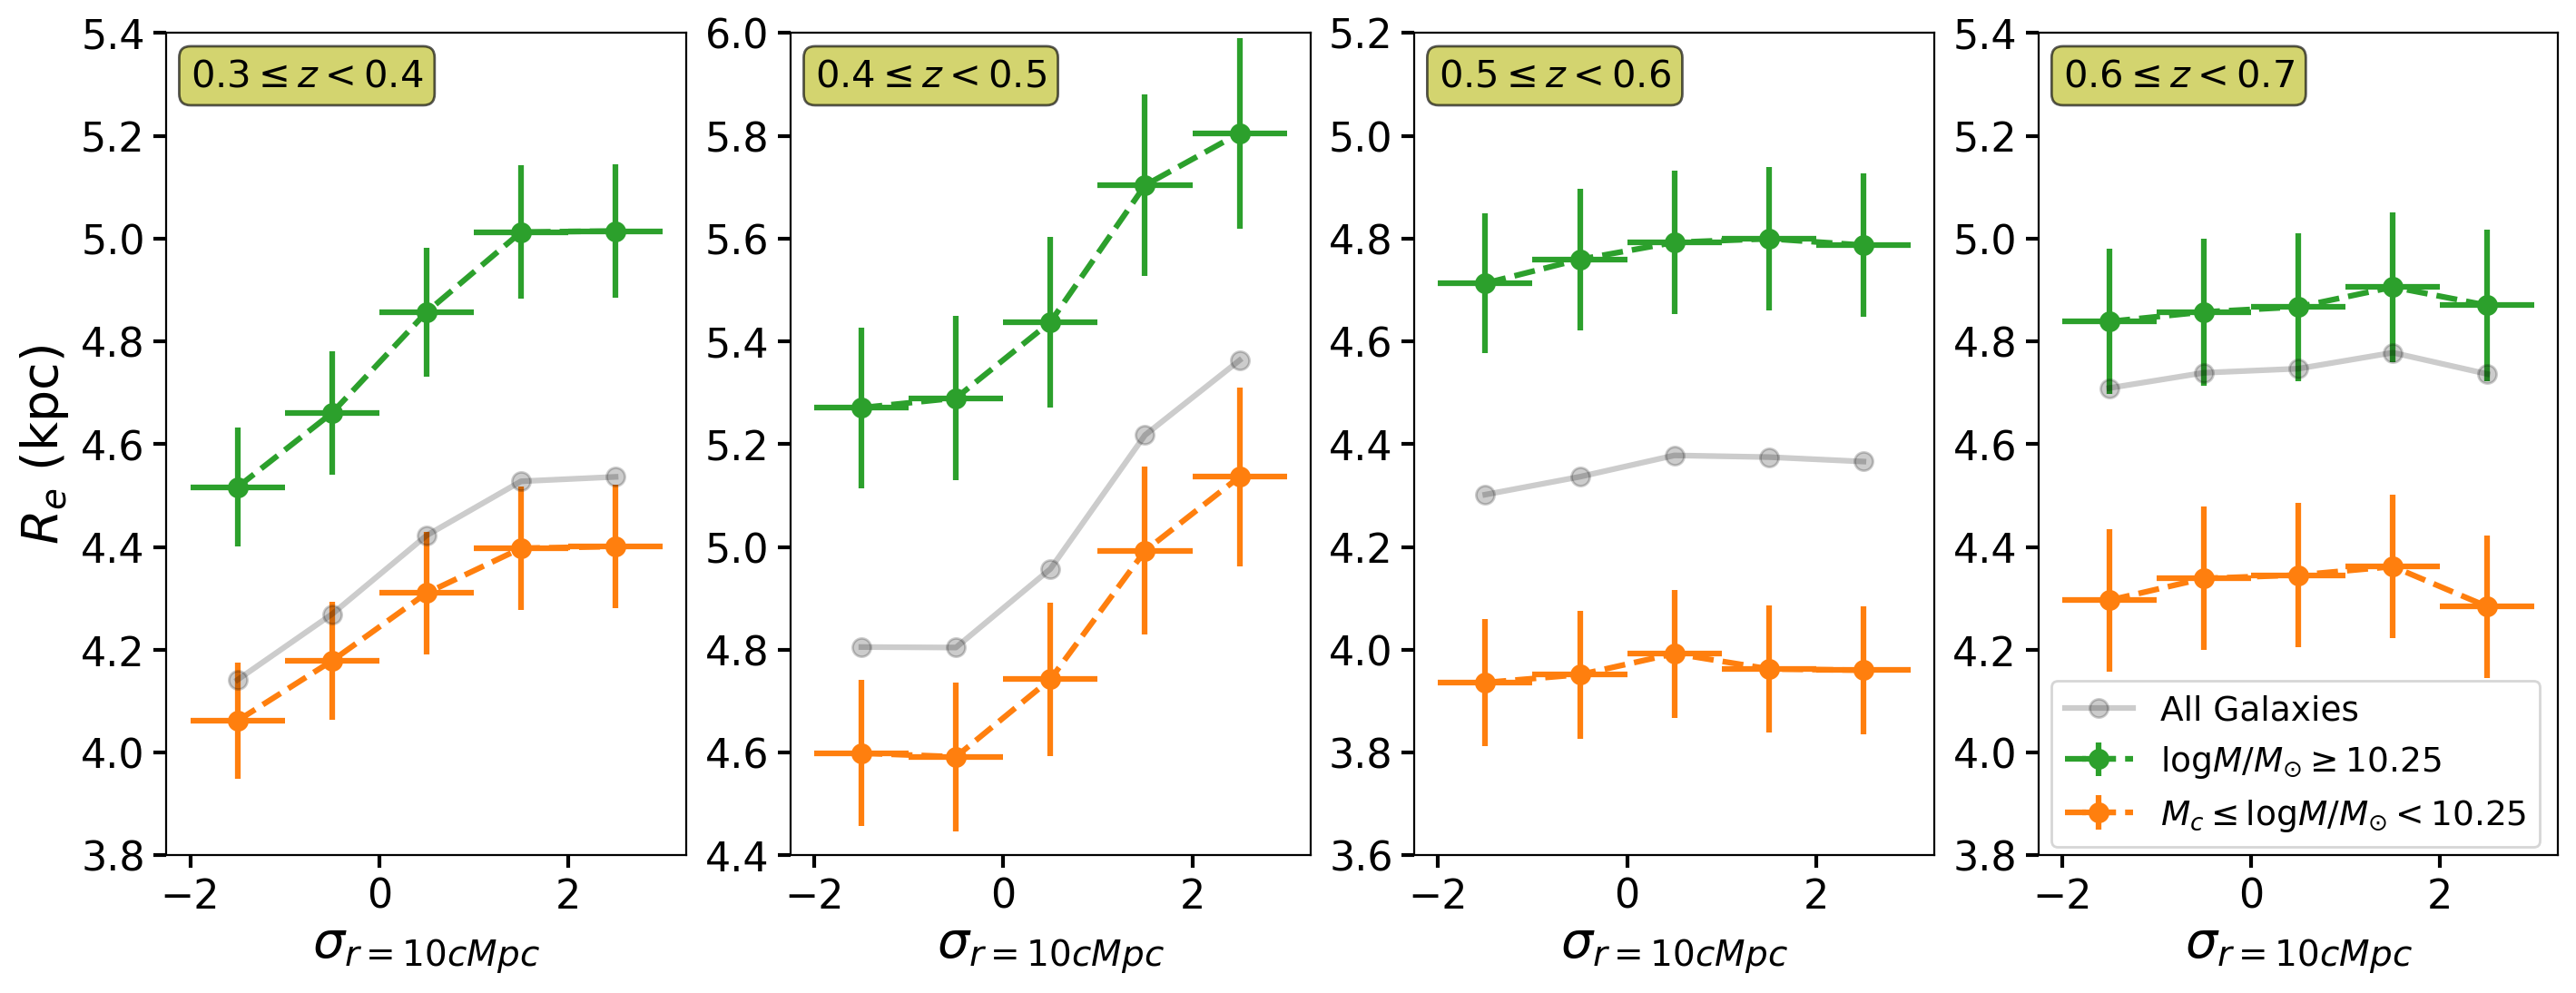
\includegraphics[width = \textwidth]{rad_den_all.png}
    \caption{The variation of effective radius with density excess is shown above, with each panel showing the relation at a different redshift slice. The different colored lines represent different stellar mass ranges, as denoted in the figure legend, with $M_c$ referring to the mass-completeness limit at the corresponding redshift. The range of densities ($-2 \leq \sigma_{r=10cMpc} < 3$) is split into five equal bins, and each point  shows the median effective radius within the corresponding bin. The vertical error bars depict the typical uncertainty (i.e., median $68\%$ confidence interval) predicted by \gampen{} for all galaxies in that bin. The gray lines depict the trend for the entire mass-complete sample. Note that although each panel shows a different $R_e$ range, the minimum $R_e$ scale of $0.2$ kpc is equal across all panels.}
    \label{fig_c4:rad_den_all}
\end{figure*}


\begin{table}
    \centering
    \caption{Measured Correlation Coefficients for Radius v/s Density Excess \label{tab_c4:corr_all}}
    \begin{tabular}{c|c|M{2.4cm}M{2.4cm}M{2.4cm}M{2.4cm}}
    \hline
    \hline 
    Mass Range & & $0.3 \leq z < 0.4$ & $0.4 \leq z < 0.5$ & $0.5 \leq z < 0.6$ & $0.6 \leq z < 0.7$ \\ 
    ($\log M/M_{\odot}$) & & & & \\
    \hline
    \hline
    \multirow[c]{3}{*}{$\geq10.25$} & $\rho$   & $1.1\times10^{-1} \pm 5.8\times10^{-4}$ & $9.6\times10^{-2} \pm 5.6\times10^{-4}$ & $1.8\times10^{-2} \pm 3.9\times10^{-4}$ & $9.7\times10^{-3} \pm 4\times10^{-4}$ \\
                                    & $p$      & $4.7\times10^{-210} \pm (<10^{-300})$ & $2.8\times10^{-205} \pm (<10^{-300})$ & $5.3\times10^{-9} \pm 5.4\times10^{-9}$ &  $2.2\times10^{-3} \pm 1.0\times10^{-3}$   \\
                                    & $\alpha$ & $184\sigma_{\rho}$ & $171\sigma_{\rho}$ & $47\sigma_{\rho}$ & $23\sigma_{\rho}$  \\
                                    & $>5\sigma$ & \checkmark & \checkmark &  Borderline \checkmark &   \\
    \hline
    \multirow{3}{*}{$\left[M_c,10.25\right)$\textsuperscript{a}} & $\rho$ & $7.7\times10^{-2} \pm 5.1\times10^{-4}$   & $1.1\times10^{-1} \pm 6.1\times10^{-4}$ & $9.7\times10^{-3} \pm 4.4\times10^{-4}$ & $2.6\times10^{-3} \pm 4.4\times10^{-4}$ \\
                                                & $p$  & $3.3\times10^{-132} \pm 1.2\times10^{-127}$ & $1.5\times10^{-232} \pm (<10^{-300})$ & $2.2\times10^{-3} \pm 1.2\times10^{-3}$ &  $4\times10^{-1} \pm 7.8\times10^{-2}$   \\
                                             & $\alpha$ & $150\sigma_{\rho}$ & $168\sigma_{\rho}$ & $21\sigma_{\rho}$ & $5\sigma_{\rho}$  \\
                                             & $>5\sigma$ & \checkmark & \checkmark &  &   \\
    \hline
    \hline
    \multicolumn{6}{p{0.95\textwidth}}{\vskip 0.01cm \small \textsuperscript{a} $M_c$ refers to the $90\%$ stellar-mass completeness limit for each corresponding redshift slice} \\
    \multicolumn{6}{p{0.95\textwidth}}{\small \texttt{NOTE-} The above table shows correlation coefficients measured using a Monte-Carlo-based Spearman's rank correlation test. The Monte-Carlo sampling technique allows us to account for uncertainties in $R_e$ measurements in our correlation analysis. $\rho$ refers to the Spearman's correlation coefficient, and $p$ refers to the probability of a spurious correlation. For both $\rho$ and $p$, median $\pm$ standard deviation values are reported above. $\alpha$ refers to the distance between the median value of $\rho$ and $\rho=0$ (signifying no correlation). It is reported above in terms of the standard deviation of $\rho$ ($\sigma_\rho$). A \checkmark indicates that we can confirm a positive correlation between $R_e$ and $\sigma_{r=10cMpc}$ with $> 5\sigma$ confidence. } \\
    \end{tabular}
\end{table}

Figure \ref{fig_c4:rad_den_all} shows the median value of the effective radius in each density bin. We also split the sample into two mass bins:-  $M_c \leq \log M/M_{\odot} < 10.25$, and $\log M/M_{\odot} \geq 10.25$. These bins were chosen as $\sim10.25M_{\odot}$ corresponds to the $75^{th}$ quantile of the overall stellar mass distribution. The vertical error bar on each point reflects the median $1\sigma$ width of the $R_e$ posterior distribution predicted by \gampen{} for all galaxies in that bin. 

Although Figure \ref{fig_c4:rad_den_all} accurately represents the available data, it does not fully capture all the information available to us. \gampen{} predicts the full posterior distribution of structural parameters, and thus, for every galaxy in our sample, we have access to the full probability distribution function of $R_e$. Therefore, judging the existence of correlations by visual inspection alone is not statistically rigorous in this scenario. Rather, we use a Monte-Carlo sampling technique to incorporate each of these predicted distributions into judging whether a correlation exists or not; and estimate with what statistical significance we can reject the null hypothesis of no correlation. 

For every galaxy in our sample, we use the predicted posterior distribution to draw 5000 samples of $R_e$, effectively creating 5000 stochastic copies of our dataset. For each of these datasets, we use the Spearman's rank correlation test \citep{spearman_original} to judge the existence of a correlation between $R_e$ and $\sigma_{r=10cMpc}$. The Spearman's test is a non-parametric method to assess how well the relationship between two variables can be described using a monotonic function. The test estimates two variables, $\rho$ and $p$. $\rho$ is the correlation coefficient that can take values between $-1$ to $+1$, with the end limits signifying the variables being perfect monotonic functions of each other. $\rho=0$ signifies no correlation between the variables. The value of $p$ roughly indicates the probability of an uncorrelated system producing datasets with a Spearman correlation at least as extreme as the computed $\rho$. The above Monte-Carlo procedure results in a distribution of $\rho$ and $p$ values for each mass bin at the four redshift slices. We refer an interested reader to Appendix \ref{sec_c4:ap:corr_coeff} for an extended description of the Monte-Carlo procedure. 

The values of the $p$ and $\rho$ obtained using the procedure above is reported in Table \ref{tab_c4:corr_all}. Note that Table \ref{tab_c4:corr_all} also reports the value of $\alpha$. We define $\alpha$ as the distance between the median value of $\rho$ and $\rho=0$ -- we report it in terms of the standard deviation ($\sigma_{\rho}$) of the $\rho$ distribution. Larger values of $\alpha$ indicate a stronger and more statistically significant correlation. The \checkmark{s} in Table \ref{tab_c4:corr_all} signify whether we can reject the null hypothesis of non-correlation at a significance level of five sigma or more. To assign a \checkmark, we verify whether $(\overline{p} + \sigma_p) < 3\times10^{-7} $ \texttt{AND} $\alpha>5\sigma_{\rho}$. Cases where $10^{-12} \leq (\overline{p} + \sigma_p) < 3\times10^{-7} $ are demarcated with ``Borderline \checkmark" to delineate them from cases where $(\overline{p} + \sigma_p) << 3\times10^{-7}$.

Table \ref{tab_c4:corr_all} and Figure \ref{fig_c4:rad_den_all} show that, for $0.3 \leq z < 0.5$, we can confirm with more than five sigma confidence, the existence of a strong positive correlation between $R_e$ and environmental density. The relationship is present across the entire mass range probed by this study, and we find that galaxies in denser environments are consistently larger than galaxies of similar mass in less dense environments. As we move to higher redshifts, the relationship significantly flattens out, with no statistically significant correlation observed for the highest redshift slice. For the $0.5 \leq z < 0.6$ slice, the observed correlations are much weaker and can be confirmed with more than five sigma confidence only for the higher-mass bin. Note that the higher mass bin always displays a marginally stronger correlation throughout our sample. 

\begin{figure*}[htb]
    \centering
    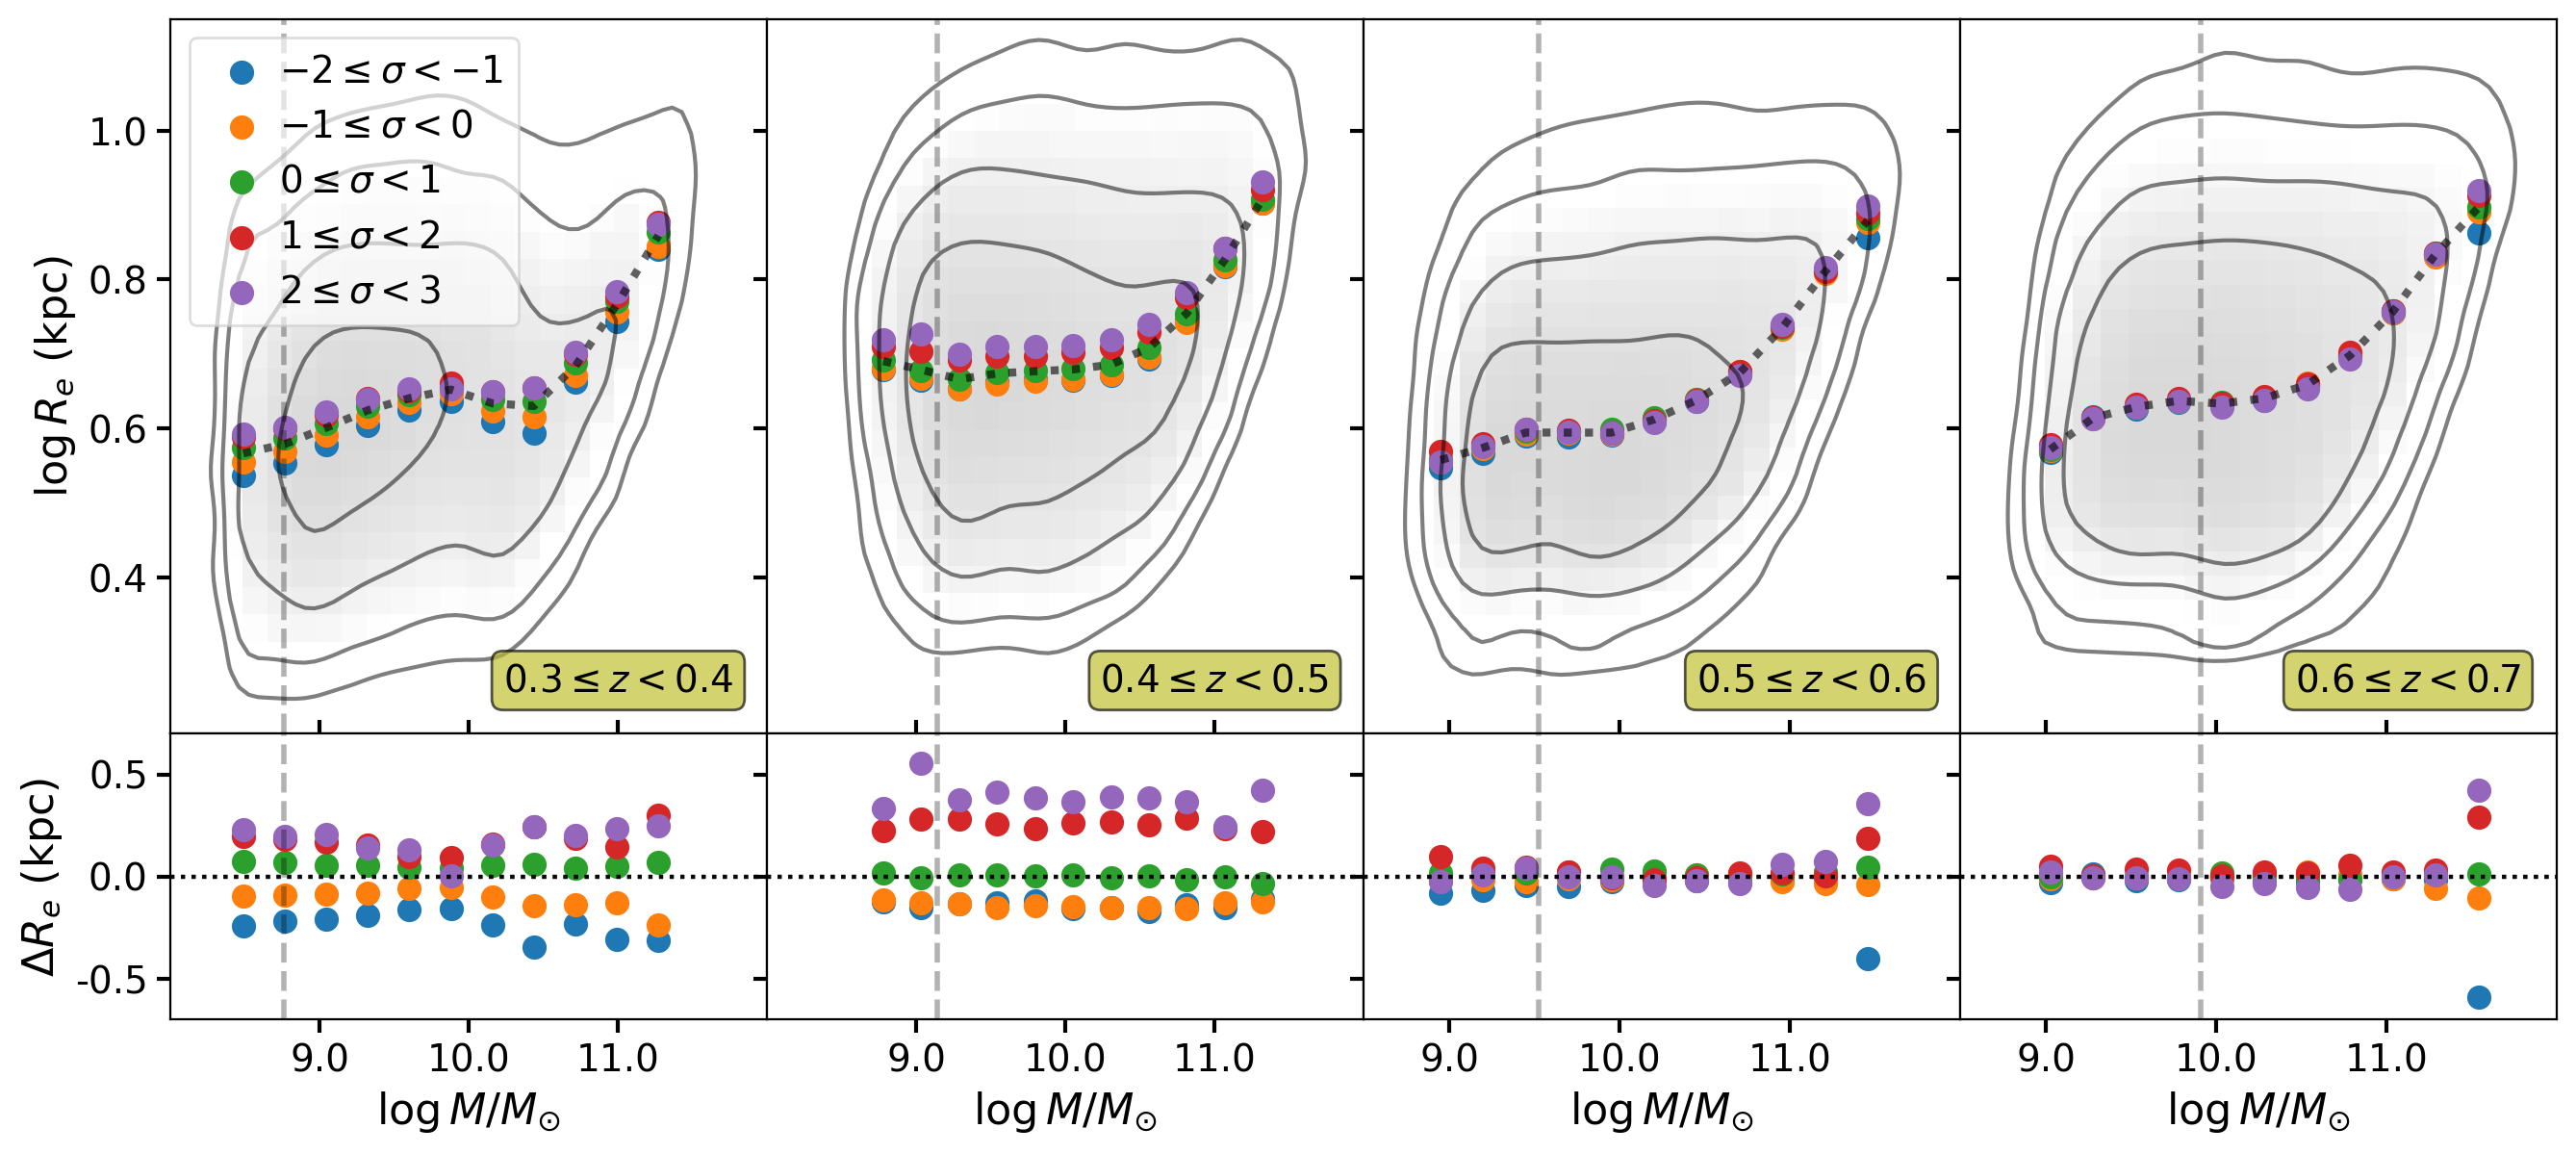
\includegraphics[width = \textwidth]{r_m_all.png}
    \caption{The size-mass relationship is shown above (top panels) for the four different redshift slices. The colored points in the top panels depict the median effective radius at a given stellar mass for all galaxies within a given density excess bin (as shown in the figure legend). The contours and shading in the top panels delineate denser regions of the size-mass plane, and the black dotted lines running alongside the colored points show the overall trend. The bottom panels show how the colored points deviate from the overall median (black-dotted) trend line. The gray dashed vertical lines running throughout the figure show the overall mass completeness in each redshift slice.}
    \label{fig_c4:r_m_all}
\end{figure*}

To investigate the variation of $R_e$ with $\sigma_{r=10cMpc}$ in finer mass bins, we plot the size-mass relationship for our sample in Figure \ref{fig_c4:r_m_all}. We investigate how galaxies with different environments are located on the size-mass plane. 
%the locations of galaxies with different environments on the size-mass plane. 
%The colored points show the median $\log(R_e)$ of galaxies in different environments at a given stellar mass. The bottom panels show how the colored points deviate from the median trend line. 
For $z < 0.5$, Figure \ref{fig_c4:r_m_all} confirms what we saw previously -- we consistently find that galaxies in denser environments are larger (by $\sim 0.5-0.7$ kpc) than galaxies of similar mass in less dense environments. For the two higher z-bins, the overall effect is much weaker/absent, consistent with what we found earlier. However, Figure \ref{fig_c4:r_m_all} adds a new dimension to our results in the $z \geq 0.5$ bins -- there appears to be a ``critical stellar mass", above which we can observe a correlation between radius and environment. The effect is significantly stronger than what can be observed for less massive galaxies at these higher redshifts. In Figure \ref{fig_c4:r_m_all}, although this effect is visible over primarily one mass bin, we have verified that when we use finer mass bins, we observe a `ramping up' of this effect for $\log M/M_{\odot} > 10^{11.25} \sim 2\times10^{11}$. We ran the Monte-Carlo correlation analysis specifically for galaxies above this critical stellar mass and observed the following values:- [$\rho = 5.5\times10^{-2} \pm 1.42\times10^{-3}$, $p = 3\times10^{-13} \pm 3.2\times10^{-12}$, $\alpha=32\sigma_{\rho}$] for the $0.5 \leq z < 0.6$ slice; and [$\rho = 5\times10^{-2} \pm 1.3\times10^{-3}$, $p = 1.4\times10^{-17} \pm 3.6\times10^{-16}$, $\alpha=36\sigma_{\rho}$] for the $0.6 \leq z < 0.7$ slice. Therefore, we have more than enough statistics at these higher masses to confirm the correlation with $>5\sigma$ confidence. Note that the existence of this high critical stellar mass might explain why some of the studies in Table \ref{tab_c4:lit_survey} did not observe any correlation at these redshifts --- many of them probably did not have enough statistics at these very high masses. 

In Figure \ref{fig_c4:r_m_all}, we also observe the existence of a mass-dependant slope of the size-mass relationship across all four redshift slices. The slope of the size-mass relationship is shallower at lower masses, with a pivotal stellar mass above which the slope becomes much steeper. This effect has been observed previously across a wide redshift range, and it has been posited that the pivotal stellar mass represents a mass above which both the stellar mass growth and the size growth of galaxies transition from being star formation dominated to dry merger dominated \citep[e.g.,][]{mowla19,hsc_mass_size}. The observed pivotal stellar masses in Figure \ref{fig_c4:r_m_all} ($\log M/M_{\odot} \sim 10.3-10.6$) are consistent with what has been observed previously, and we can additionally confirm that the pivotal stellar mass does not appear to be dependent on environmental density. 


\subsubsection{Specific Sub-Populations} \label{sec_c4:rad_den_sub}

%\begin{figure*}[htb]
%    \centering
%    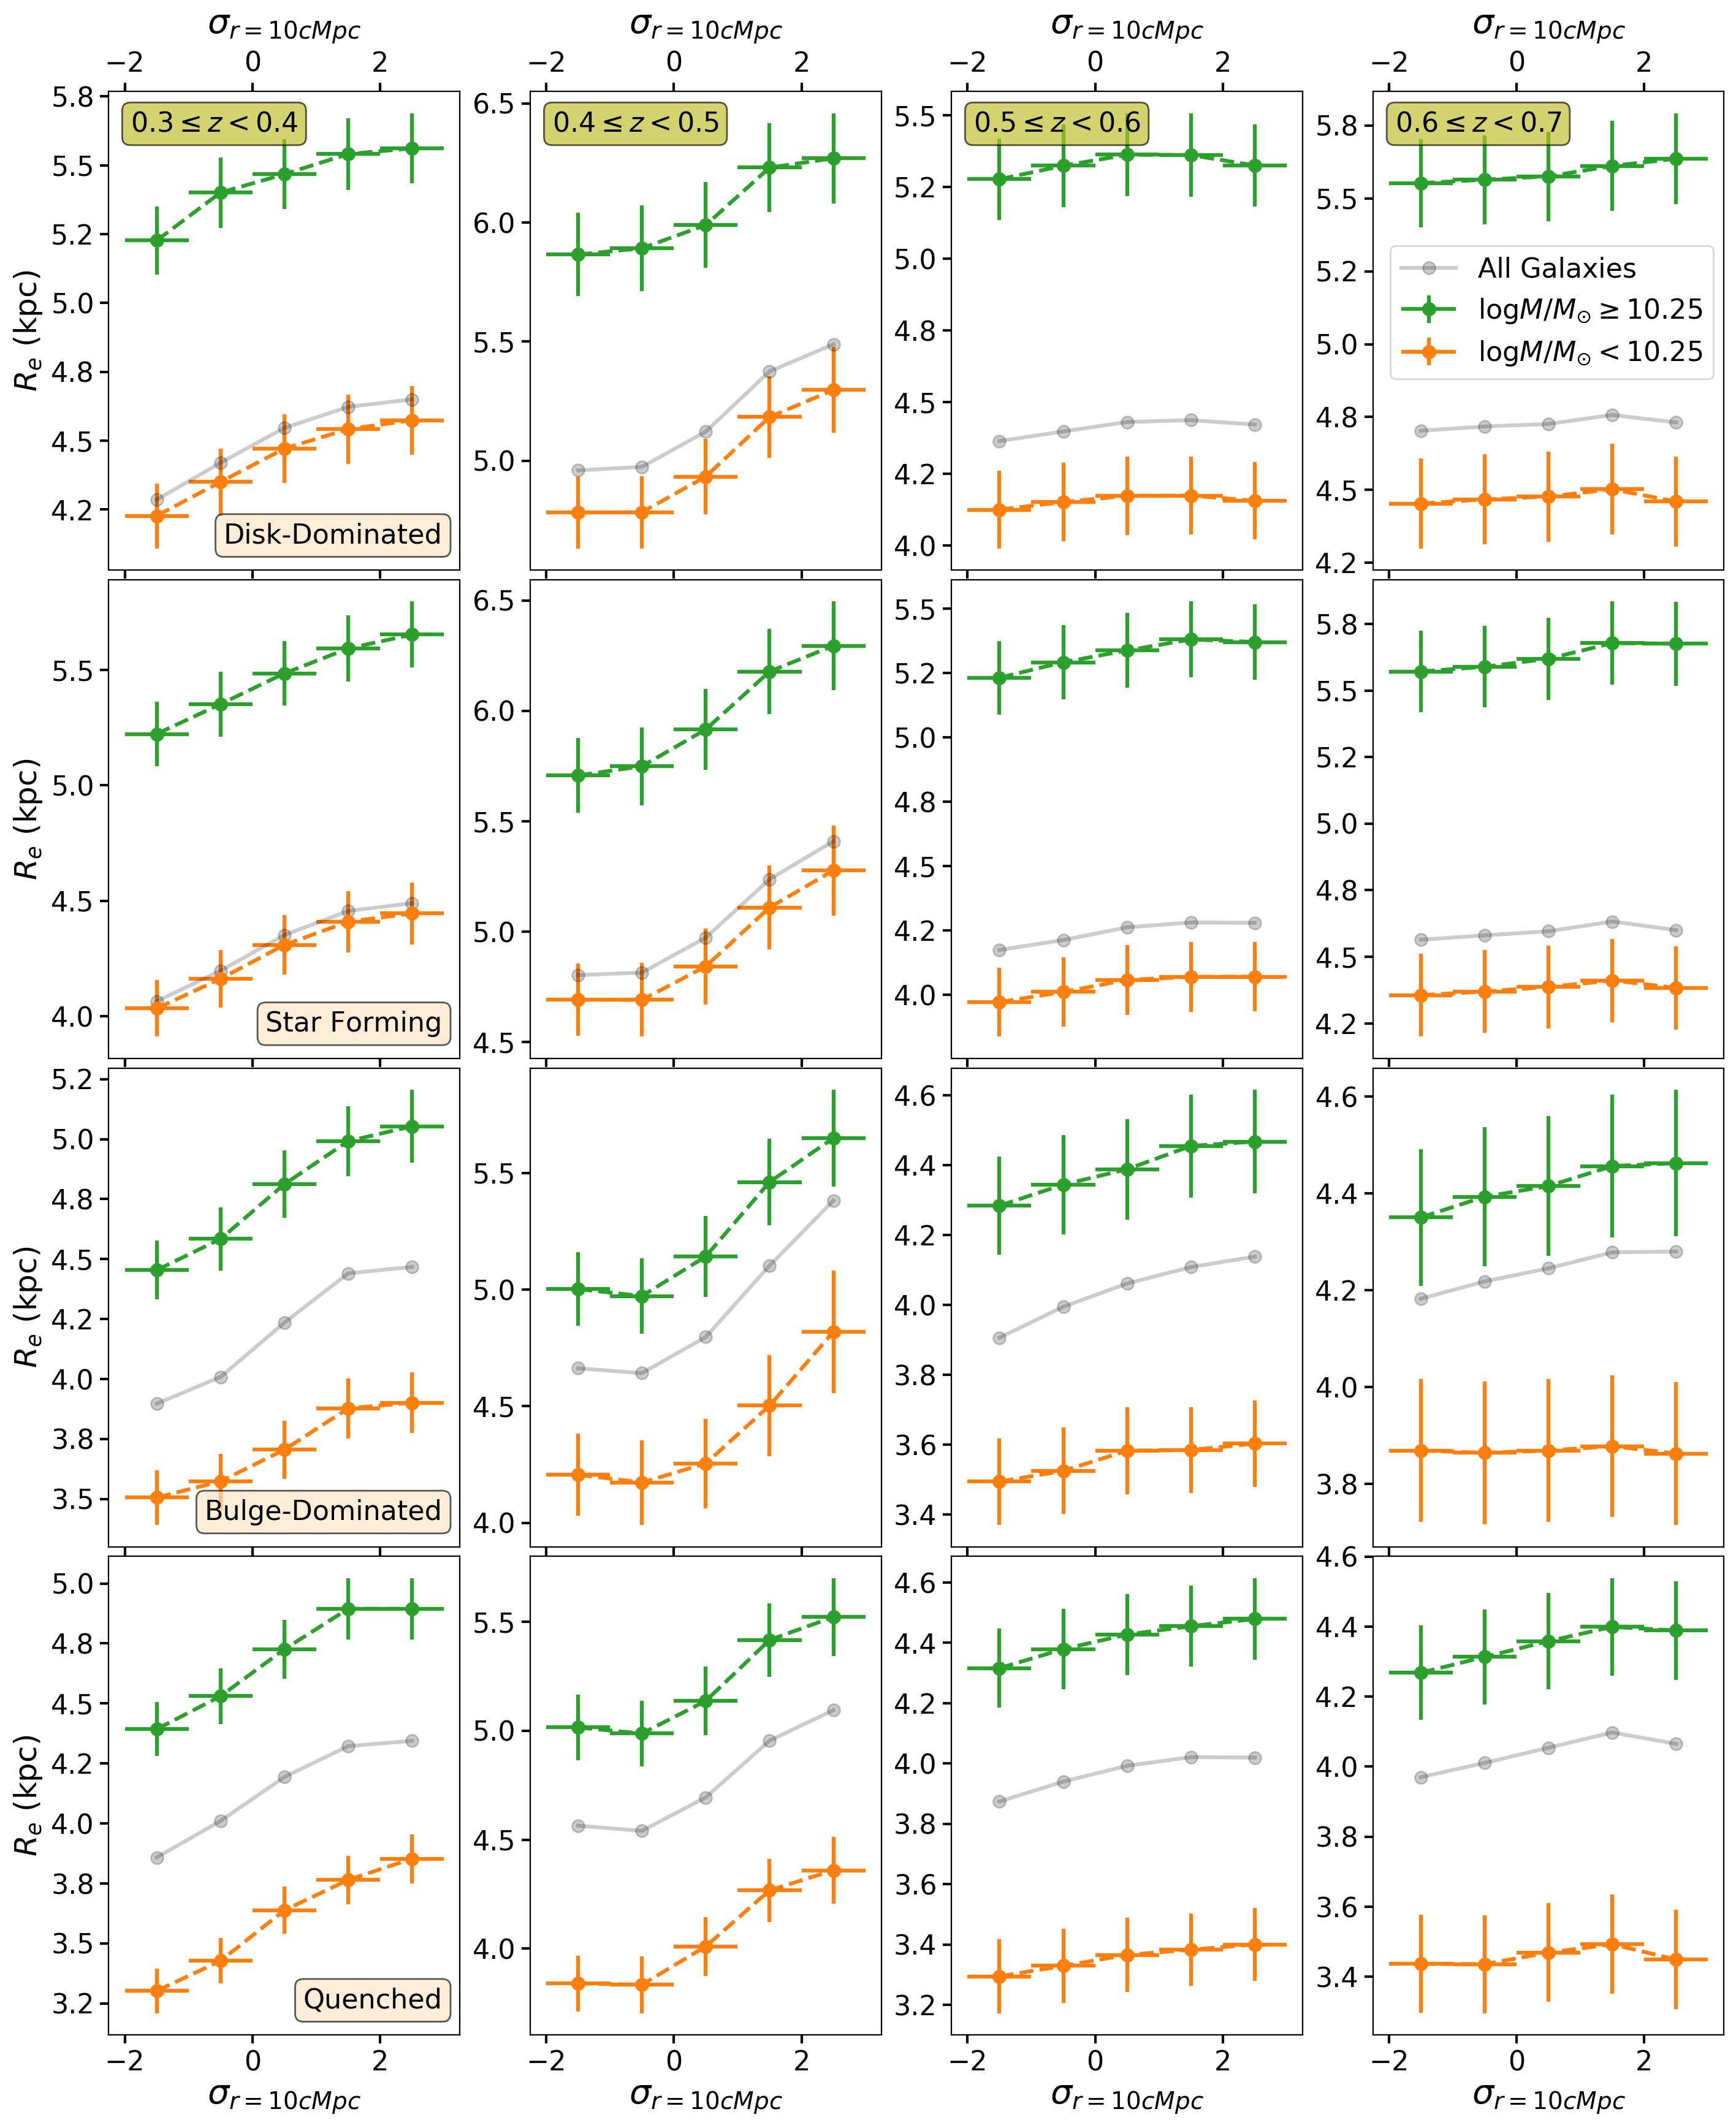
\includegraphics[width = 0.85\textwidth]{rad_den_sub.png}
%    \caption{Effective radius v/s density excess at different redshifts (different columns) shown for different sub-samples of galaxies (different rows). The points show the median radius in each bin and the error bars depict the median $68\%$ confidence interval predicted by \gampen{} for all galaxies in that bin. The grey line shows the median trend for the entire sample in the given redshift bin. Note that we merged the two lower mass bins used in Figure \ref{fig_c4:rad_den_all} into one bin in this Figure to ensure statistically significant sample sizes in each measurement bin.}
%    \label{fig_c4:rad_den_sub}
%\end{figure*}

\begin{figure*}
    \begin{center}
        \subfigure{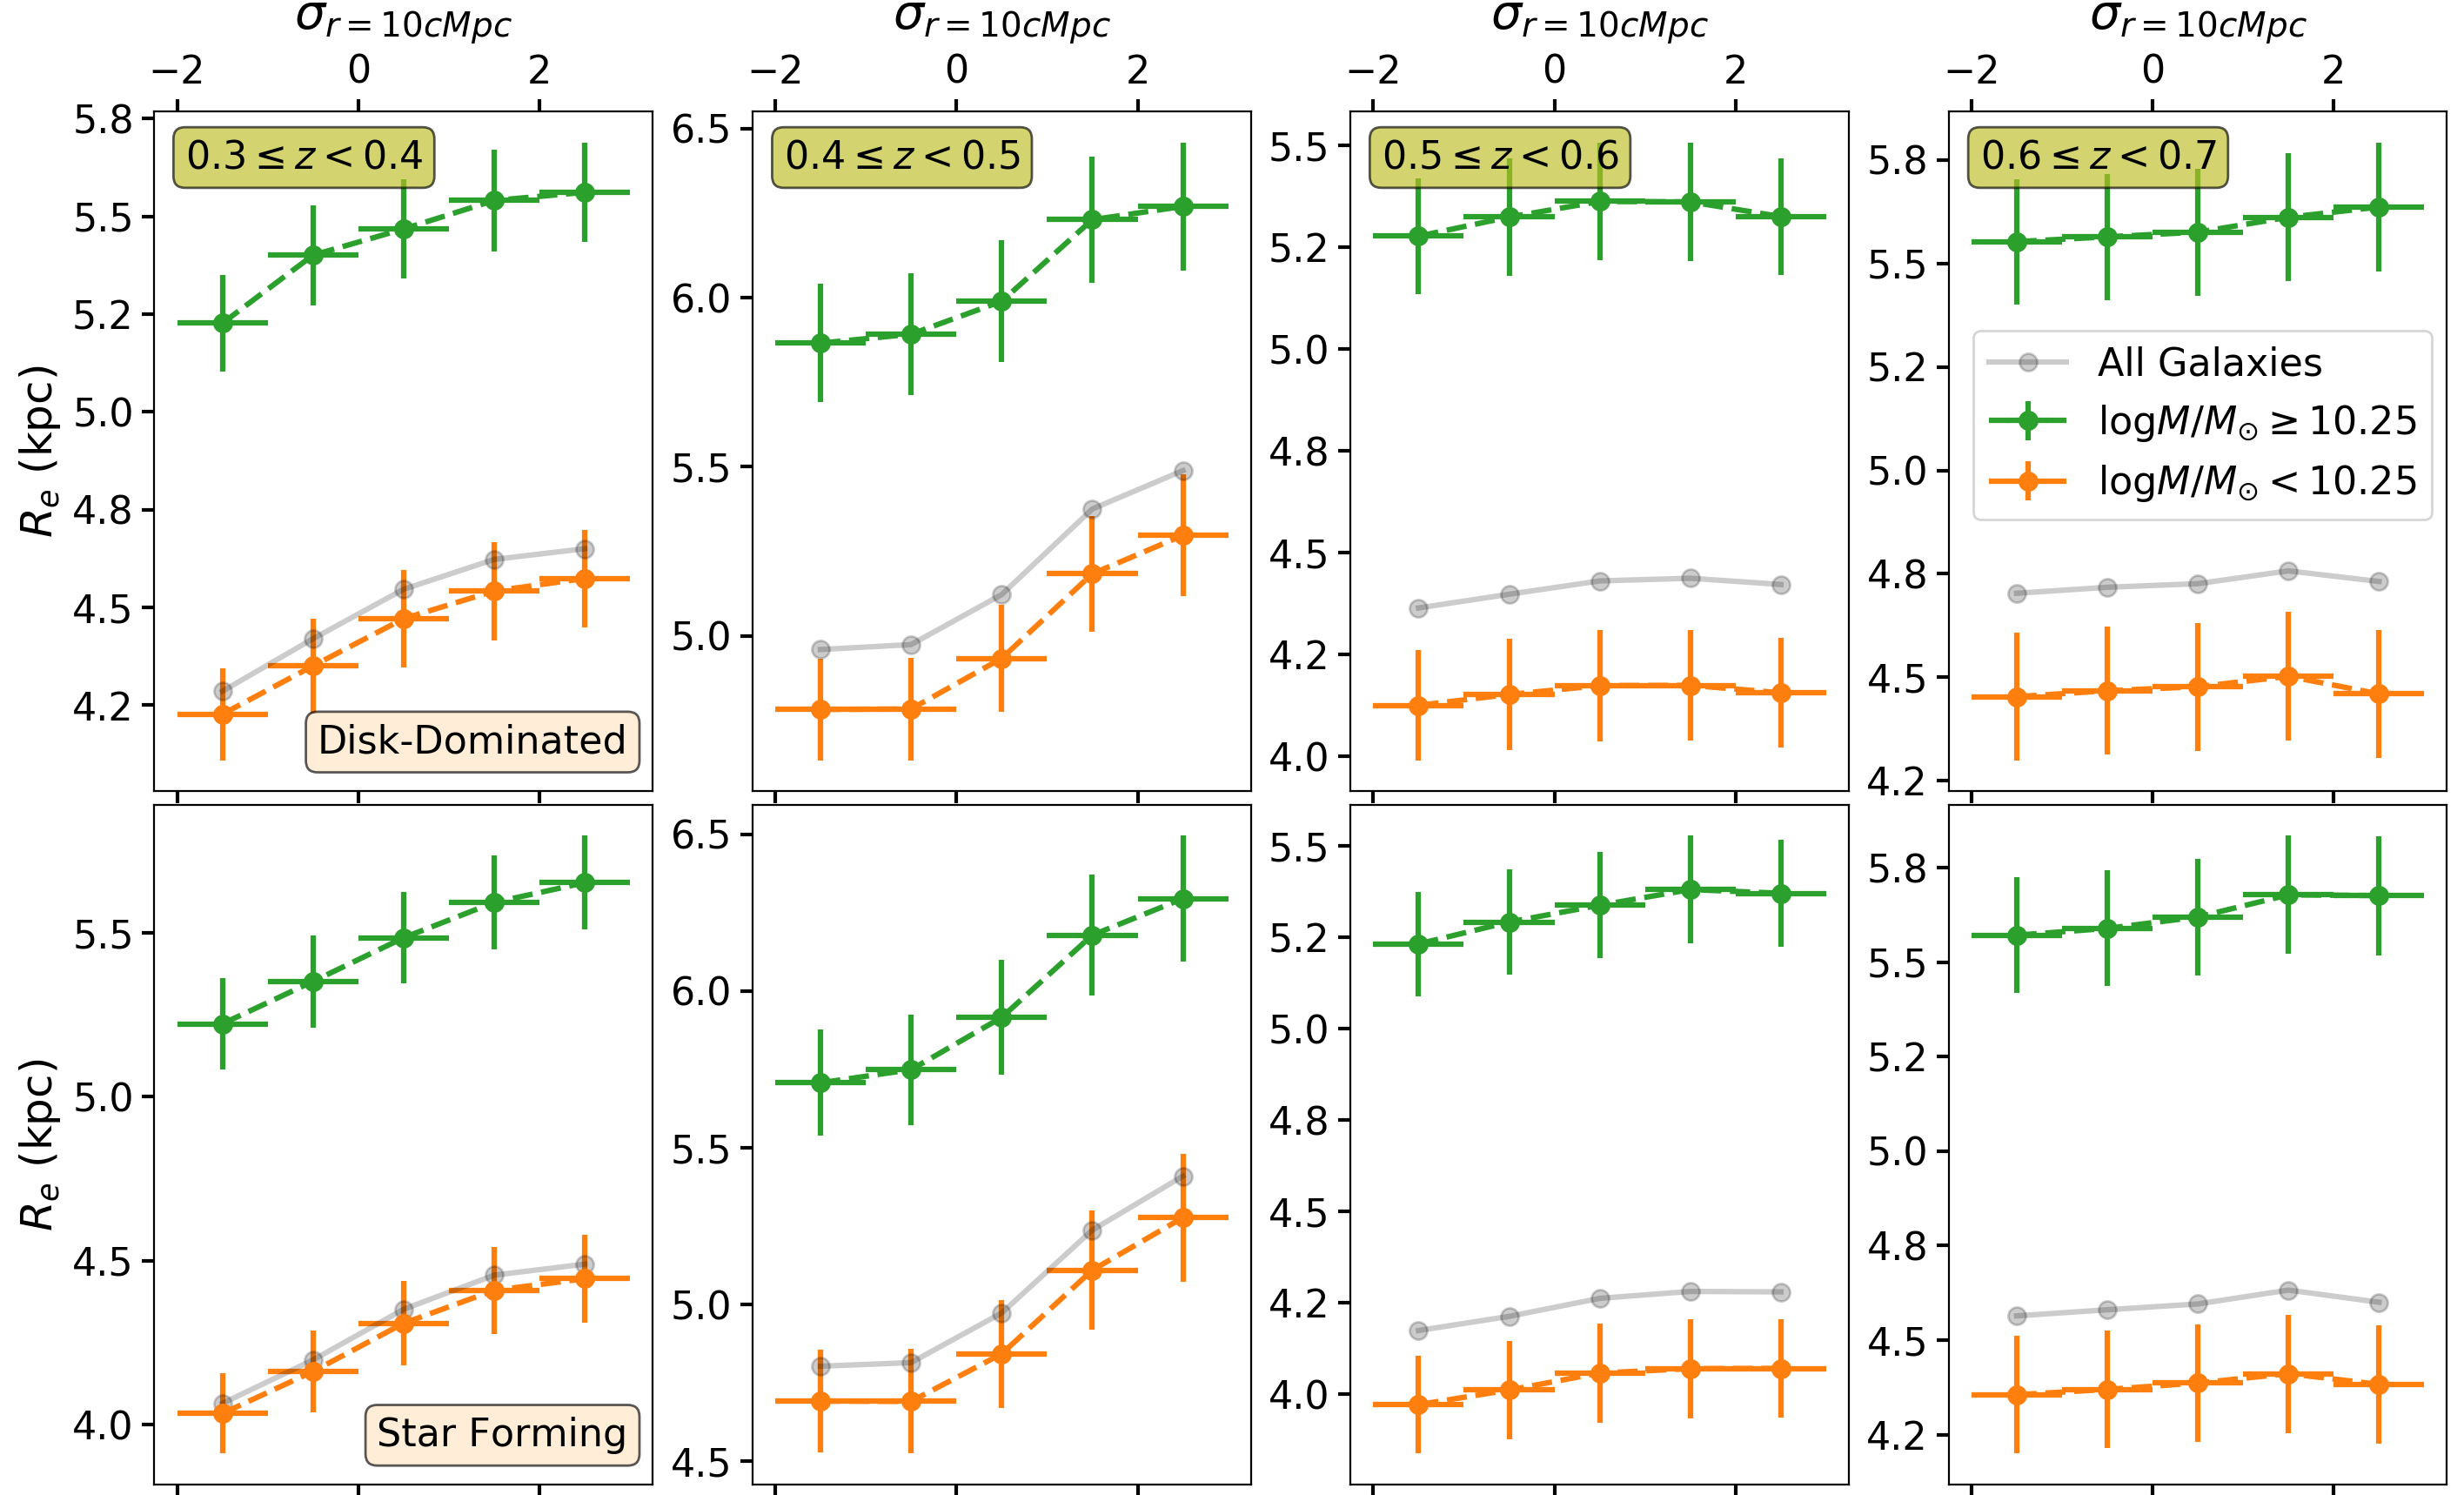
\includegraphics[width=\textwidth]{rad_den_sub_1.png}} 
        \subfigure{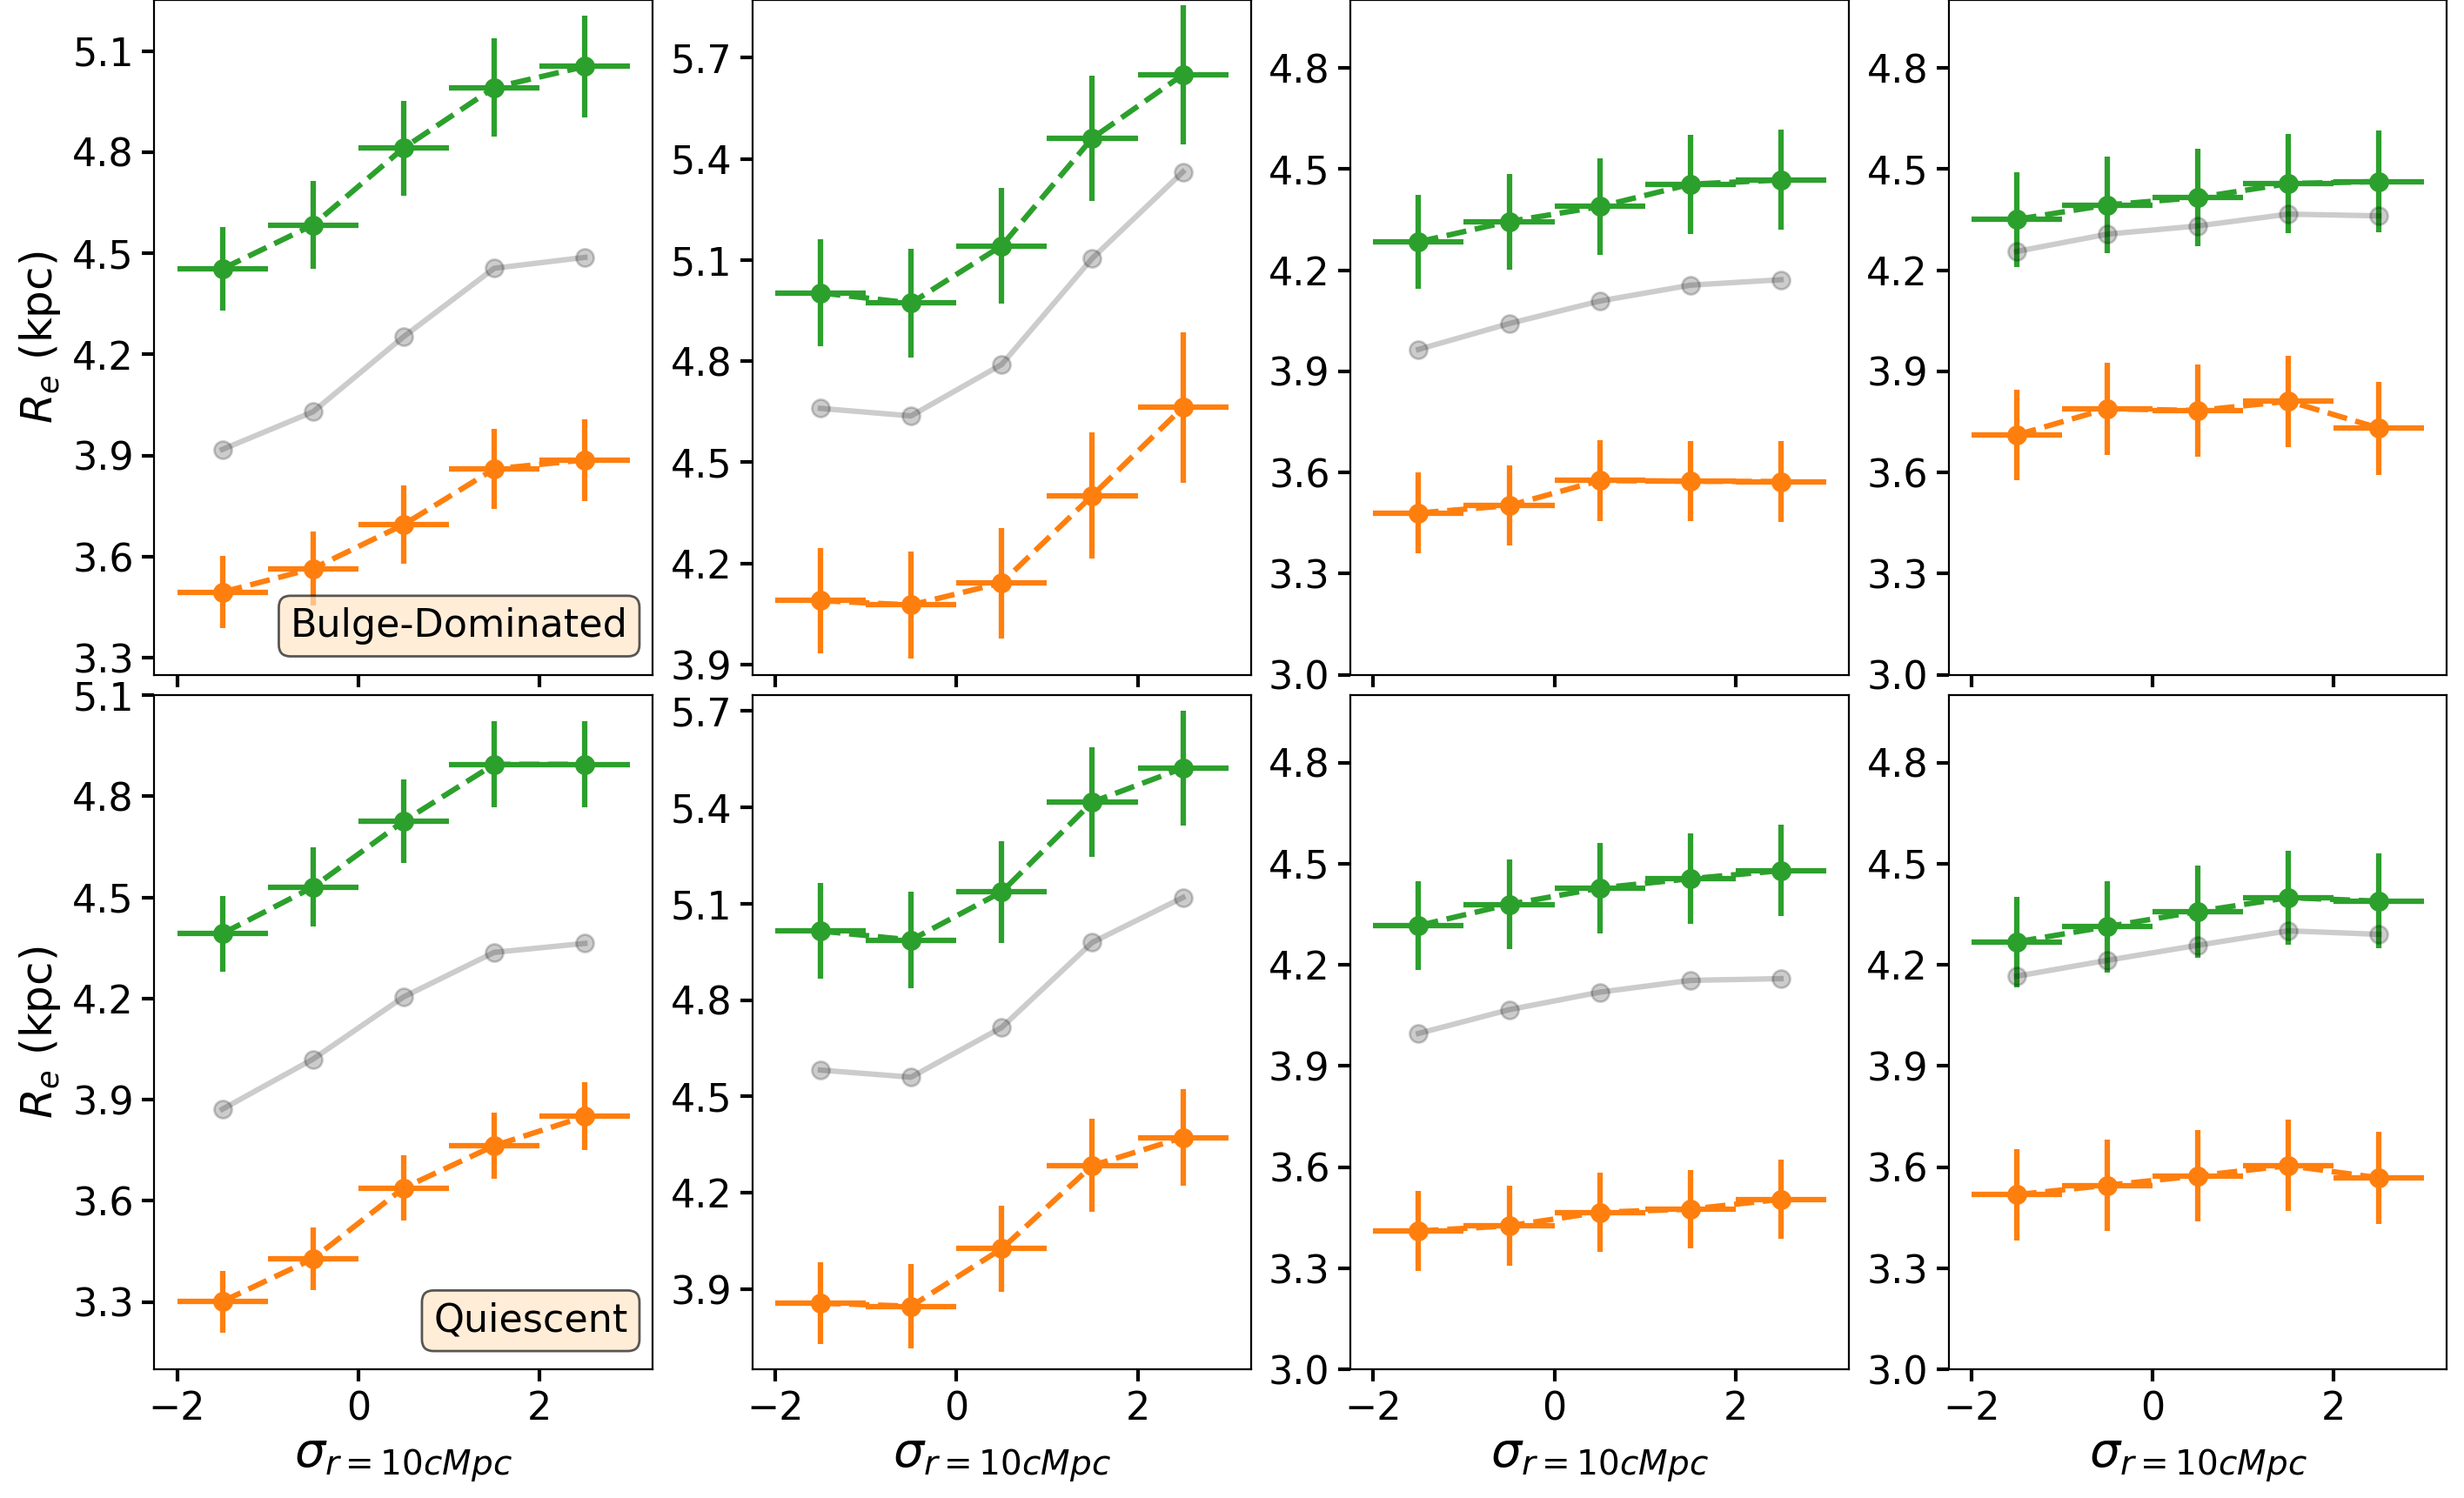
\includegraphics[width=\textwidth]{rad_den_sub_2.png}} 
  \end{center}
  \caption{The variation of effective radius with density excess is shown above for different sub-populations of galaxies (four rows) at different redshifts (four columns). The different colored lines represent different stellar mass ranges as denoted in the figure legend, with $M_c$ referring to the mass-completeness limit at the corresponding redshift. The points depict the median effective radius in each density bin and vertical error bars show the typical uncertainty (i.e., median $68\%$ confidence interval) predicted by \gampen{} for all galaxies in that bin. The gray lines depict the trend for the entire mass-complete sample. Note that although each panel shows a different $R_e$ range, the minimum $R_e$ scale of $0.3$ kpc is equal across all panels.}
    \label{fig_c4:rad_den_sub}
\end{figure*}

\begin{table}
    \centering
    \caption{Radius v/s Density Correlation Coefficients for Different Sub-Populations  \label{tab_c4:corr_subpop_ab}}
    \begin{tabular}{>{\centering\arraybackslash}p{2cm}|c|c|cccc}
        \hline
        \hline
        Sub-Population & Mass Range & & $0.3 \leq z < 0.4$ & $0.4 \leq z < 0.5$ & $0.5 \leq z < 0.6$ & $0.6 \leq z < 0.7$ \\ 
          & ($\log M/M_{\odot}$) & & & & \\
        \hline
        \hline 
    \multirow{8}{*}{Disk-Dom.} & \multirow[c]{4}{*}{$\geq10.25$} & $\rho$   & $\om(10^{-2})$ & $\om(10^{-2})$ & $\om(10^{-2})$ & $\om(10^{-2})$ \\
                                    &                                  & $p$      & $\om(10^{-13})$ & $\om(10^{-101})$ & $\om(10^{-10})$ &  $\om(10^{-7})$   \\
                                    &                                  & $\alpha$ & $48\sigma_{\rho}$ & $90\sigma_{\rho}$ & $48\sigma_{\rho}$ & $37\sigma_{\rho}$  \\
                                    & & $>5\sigma$ & \checkmark & \checkmark &  Borderline \checkmark &   \\
                 \cline{2-7}
                 & \multirow[c]{4}{*}{$\left[M_c,10.25\right)$\textsuperscript{a}} & $\rho$   & $\om(10^{-2})$ & $\om(10^{-1})$ & $\om(10^{-3})$ & $\om(10^{-2})$ \\
                                    &             & $p$                    & $\om(10^{-103})$ & $\om(10^{-224})$ & $\om(10^{-2})$ &  $\om(10^{-3})$   \\
                                    & & $\alpha$                           & $145\sigma_{\rho}$ & $187\sigma_{\rho}$ & $18\sigma_{\rho}$ & $16\sigma_{\rho}$  \\
                                    & & $>5\sigma$ & \checkmark & \checkmark &  &  \\
    \hline
    \hline
    \multirow{8}{*}{Star-Forming} & \multirow[c]{4}{*}{$\geq10.25$}       & $\rho$   & $\om(10^{-2})$ & $\om(10^{-1})$ & $\om(10^{-2})$ & $\om(10^{-2})$ \\
                                    &                                     & $p$      & $\om(10^{-18})$ & $\om(10^{-160})$ & $\om(10^{-20})$ &  $\om(10^{-12})$   \\
                                    &                                     & $\alpha$ & $48\sigma_{\rho}$ & $110\sigma_{\rho}$ & $42\sigma_{\rho}$ & $50\sigma_{\rho}$  \\
                                    & & $>5\sigma$ & \checkmark & \checkmark & \checkmark &  Borderline \checkmark \\
                 \cline{2-7}
                 & \multirow[c]{4}{*}{$\left[M_c,10.25\right)$} & $\rho$   & $\om(10^{-2})$ & $\om(10^{-1})$ & $\om(10^{-2})$ & $\om(10^{-2})$ \\
                                    &             & $p$                    & $\om(10^{-135})$ & $\om(10^{-265})$ & $\om(10^{-15})$ &  $\om(10^{-9})$   \\
                                    & & $\alpha$                           & $144\sigma_{\rho}$ & $170\sigma_{\rho}$ & $55\sigma_{\rho}$ & $40\sigma_{\rho}$  \\
                                    & & $>5\sigma$ & \checkmark & \checkmark & \checkmark & Borderline \checkmark \\
    \hline
    \hline
    \multirow{8}{*}{Bulge-Dom.} & \multirow[c]{4}{*}{$\geq10.25$} & $\rho$   & $\om(10^{-1})$ & $\om(10^{-1})$ & $\om(10^{-2})$ & $\om(10^{-2})$ \\
                                    &                                     & $p$   & $\om(10^{-155})$ & $\om(10^{-168})$ & $\om(10^{-42})$ &  $\om(10^{-22})$   \\
                                    & & $\alpha$                                  & $134\sigma_{\rho}$ & $122\sigma_{\rho}$ & $52\sigma_{\rho}$ & $58\sigma_{\rho}$  \\
                                    & & $>5\sigma$ & \checkmark & \checkmark &  \checkmark &  \checkmark \\
                 \cline{2-7}
                 & \multirow[c]{4}{*}{$\left[M_c,10.25\right)$} & $\rho$    & $\om(10^{-1})$ & $\om(10^{-2})$ & $\om(10^{-2})$ & $\om(10^{-3})$ \\
                                    &             & $p$                     & $\om(10^{-92})$ & $\om(10^{-35})$ & $\om(10^{-23})$ &  $\om(10^{-1})$   \\
                                    & & $\alpha$                            & $82\sigma_{\rho}$ & $42\sigma_{\rho}$ & $29\sigma_{\rho}$ & $3\sigma_{\rho}$  \\
                                    & & $>5\sigma$ & \checkmark & \checkmark & \checkmark &  \\
    \hline
    \hline
    \multirow{8}{*}{Quiescent} & \multirow[c]{4}{*}{$\geq10.25$} & $\rho$   & $\om(10^{-1})$ & $\om(10^{-1})$ & $\om(10^{-2})$ & $\om(10^{-2})$ \\
                                    &                            & $p$      & $\om(10^{-197})$ & $\om(10^{-226})$ & $\om(10^{-28})$ &  $\om(10^{-23})$   \\
                                    &                            & $\alpha$ & $177\sigma_{\rho}$ & $189\sigma_{\rho}$ & $84\sigma_{\rho}$ & $74\sigma_{\rho}$  \\
                                    & & $>5\sigma$  & \checkmark & \checkmark &  \checkmark &  \checkmark \\
                 \cline{2-7}
                 & \multirow[c]{4}{*}{$\left[M_c,10.25\right)$} & $\rho$   & $\om(10^{-1})$ & $\om(10^{-1})$ & $\om(10^{-2})$ & $\om(10^{-2})$ \\
                                    &             & $p$                    & $\om(10^{-250})$ & $\om(10^{-228})$ & $\om(10^{-17})$ &  $\om(10^{-5})$   \\
                                    &     & $\alpha$                       & $157\sigma_{\rho}$ & $131\sigma_{\rho}$ & $24\sigma_{\rho}$ & 13$\sigma_{\rho}$  \\
                                    & & $>5\sigma$  & \checkmark & \checkmark & \checkmark & \\
        \hline
        \hline
        \multicolumn{7}{p{0.99\textwidth}}{\vskip 0.01cm \small \textsuperscript{a} $M_c$ refers to the $90\%$ stellar-mass completeness limit for each corresponding redshift slice} \\
    \multicolumn{7}{p{0.99\textwidth}}{\small \texttt{NOTE-} The above table shows correlation coefficients measured using a Monte-Carlo-based Spearman's rank correlation test for different sub-populations of galaxies. The format of the table and the variables used are identical to that of Table \ref{tab_c4:corr_all}. For formatting constraints, we only report median order-of-magnitude values for $\rho$ and $p$. The unabridged version of this table, presented in Appendix \ref{sec_c4:ap:corr_coeff}, reports the full median and standard deviation values. A \checkmark indicates that we can confirm a positive correlation between $R_e$ and $\sigma_{r=10cMpc}$ with $> 5\sigma$ confidence.} \\
    \end{tabular}
\end{table}


\begin{figure*}
    \begin{center}
        \subfigure{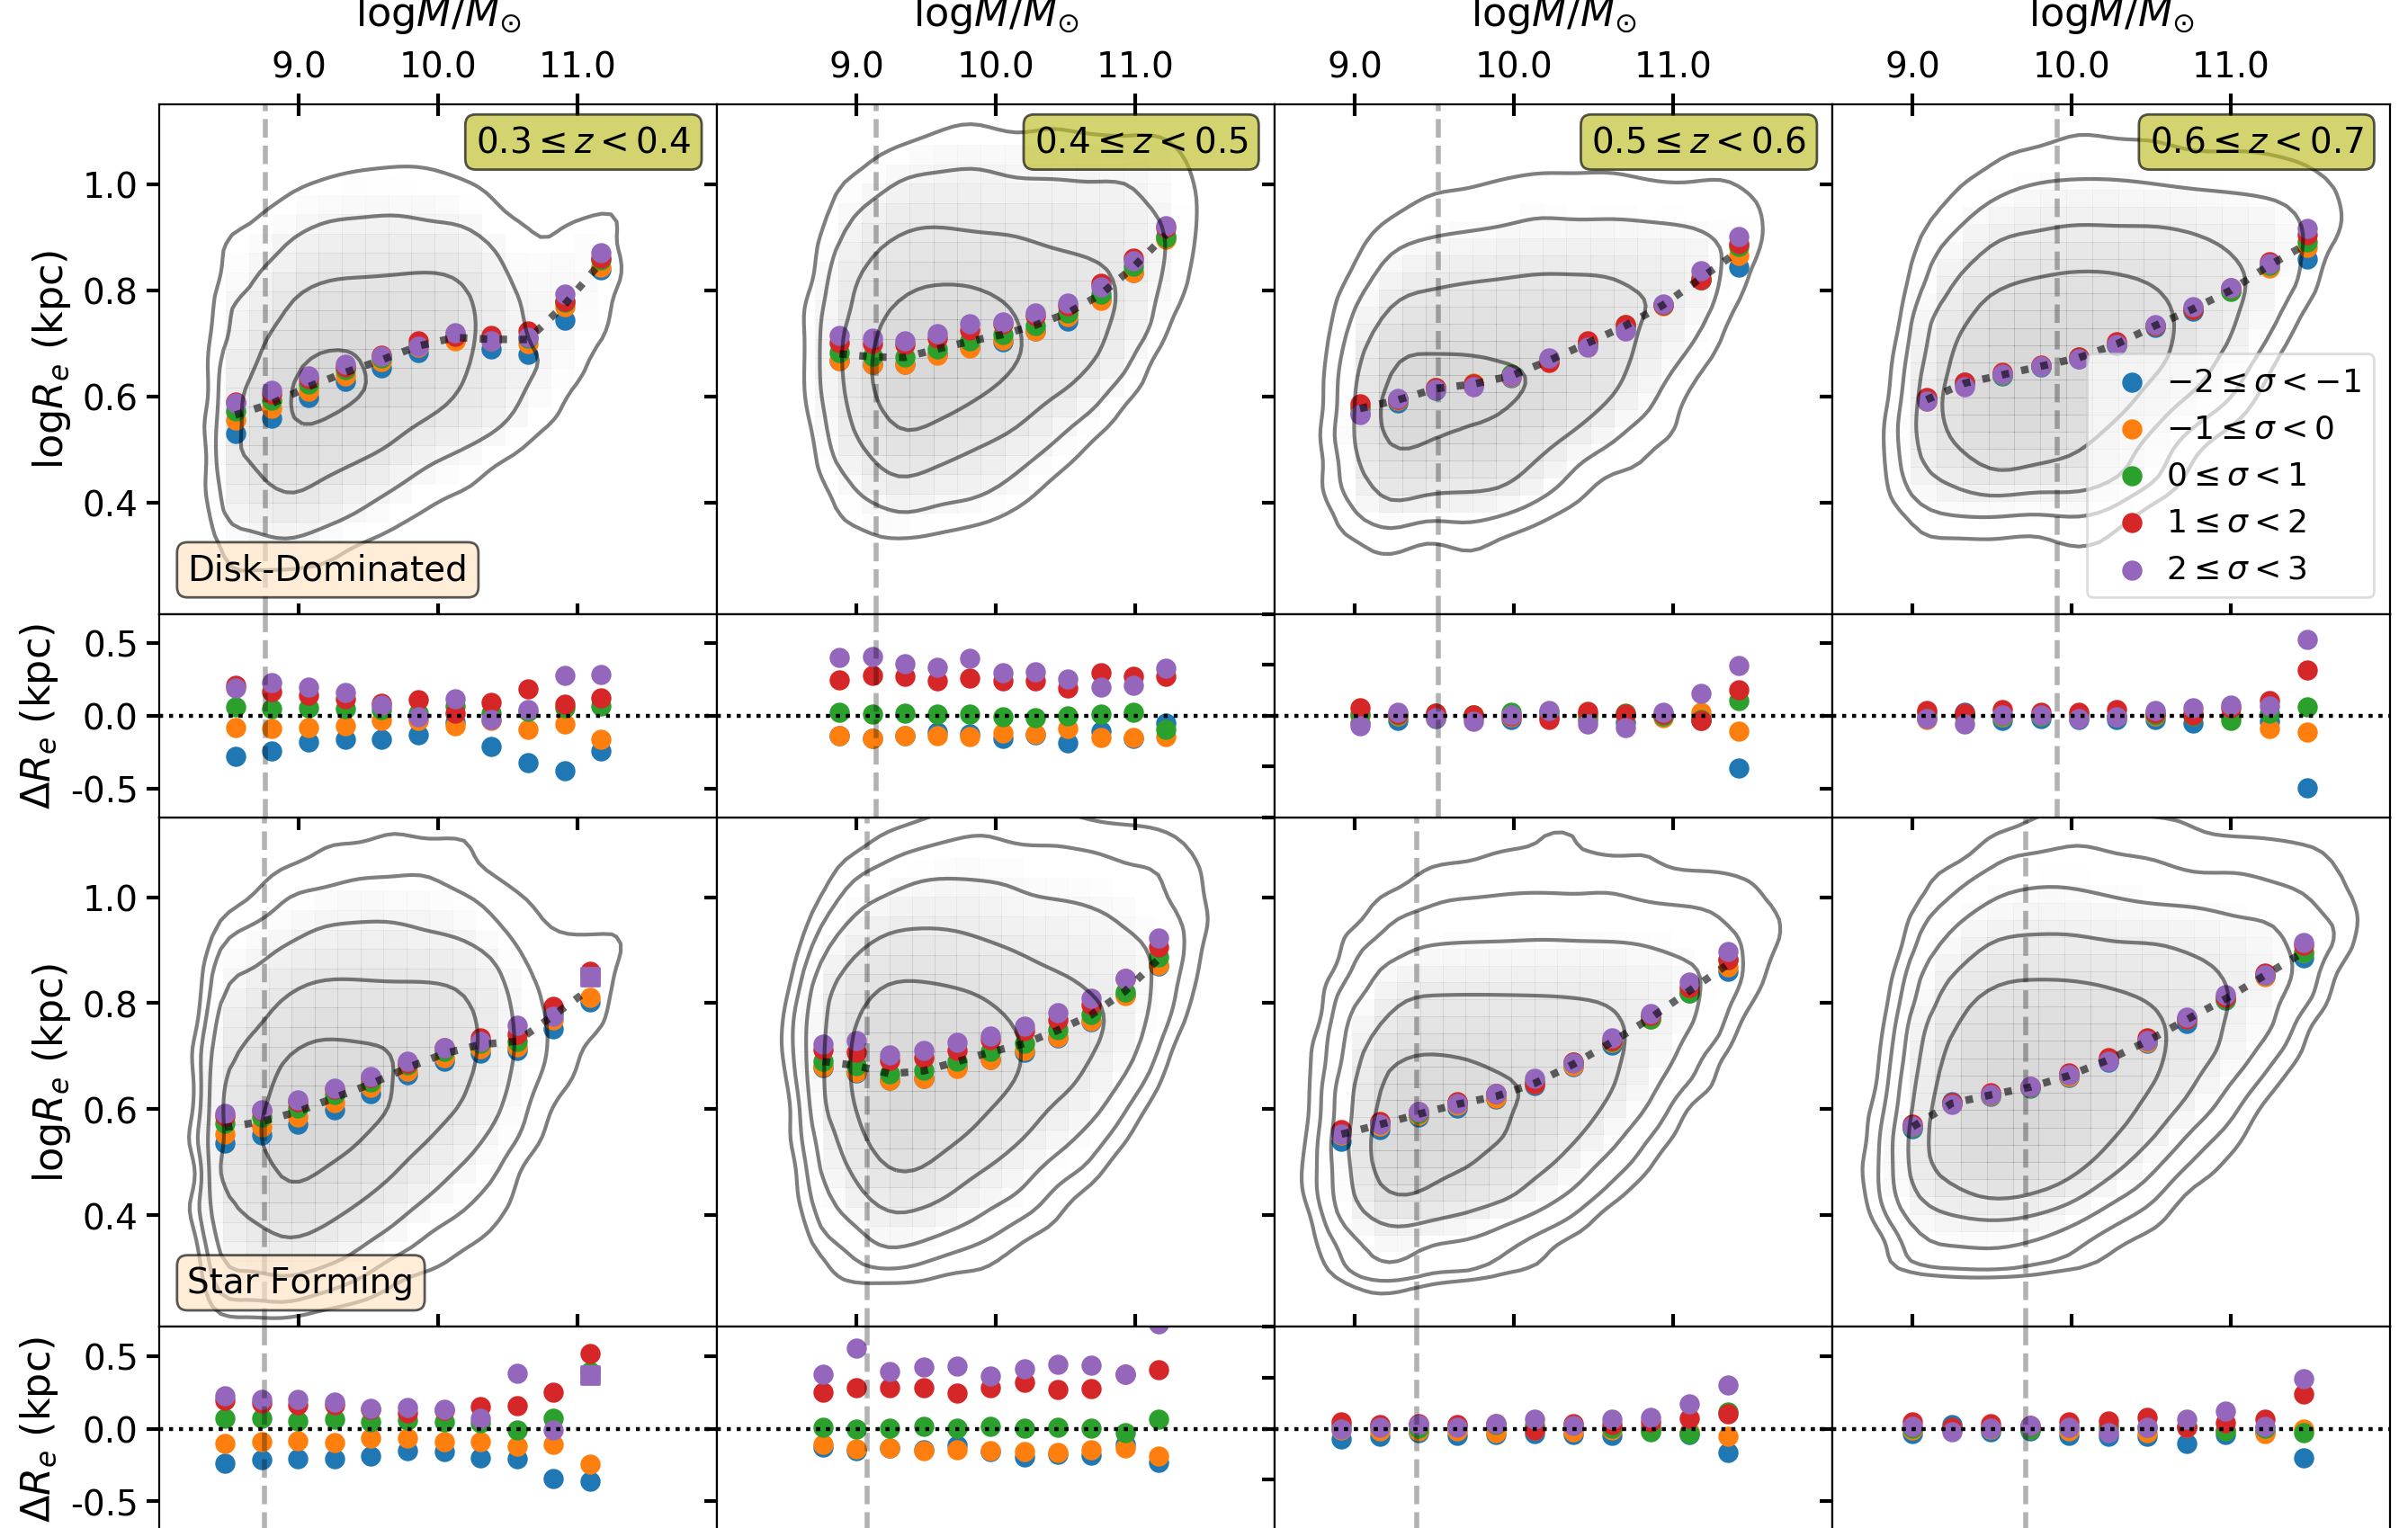
\includegraphics[width=0.95\textwidth]{r_m_sub_1.png}} 
        \subfigure{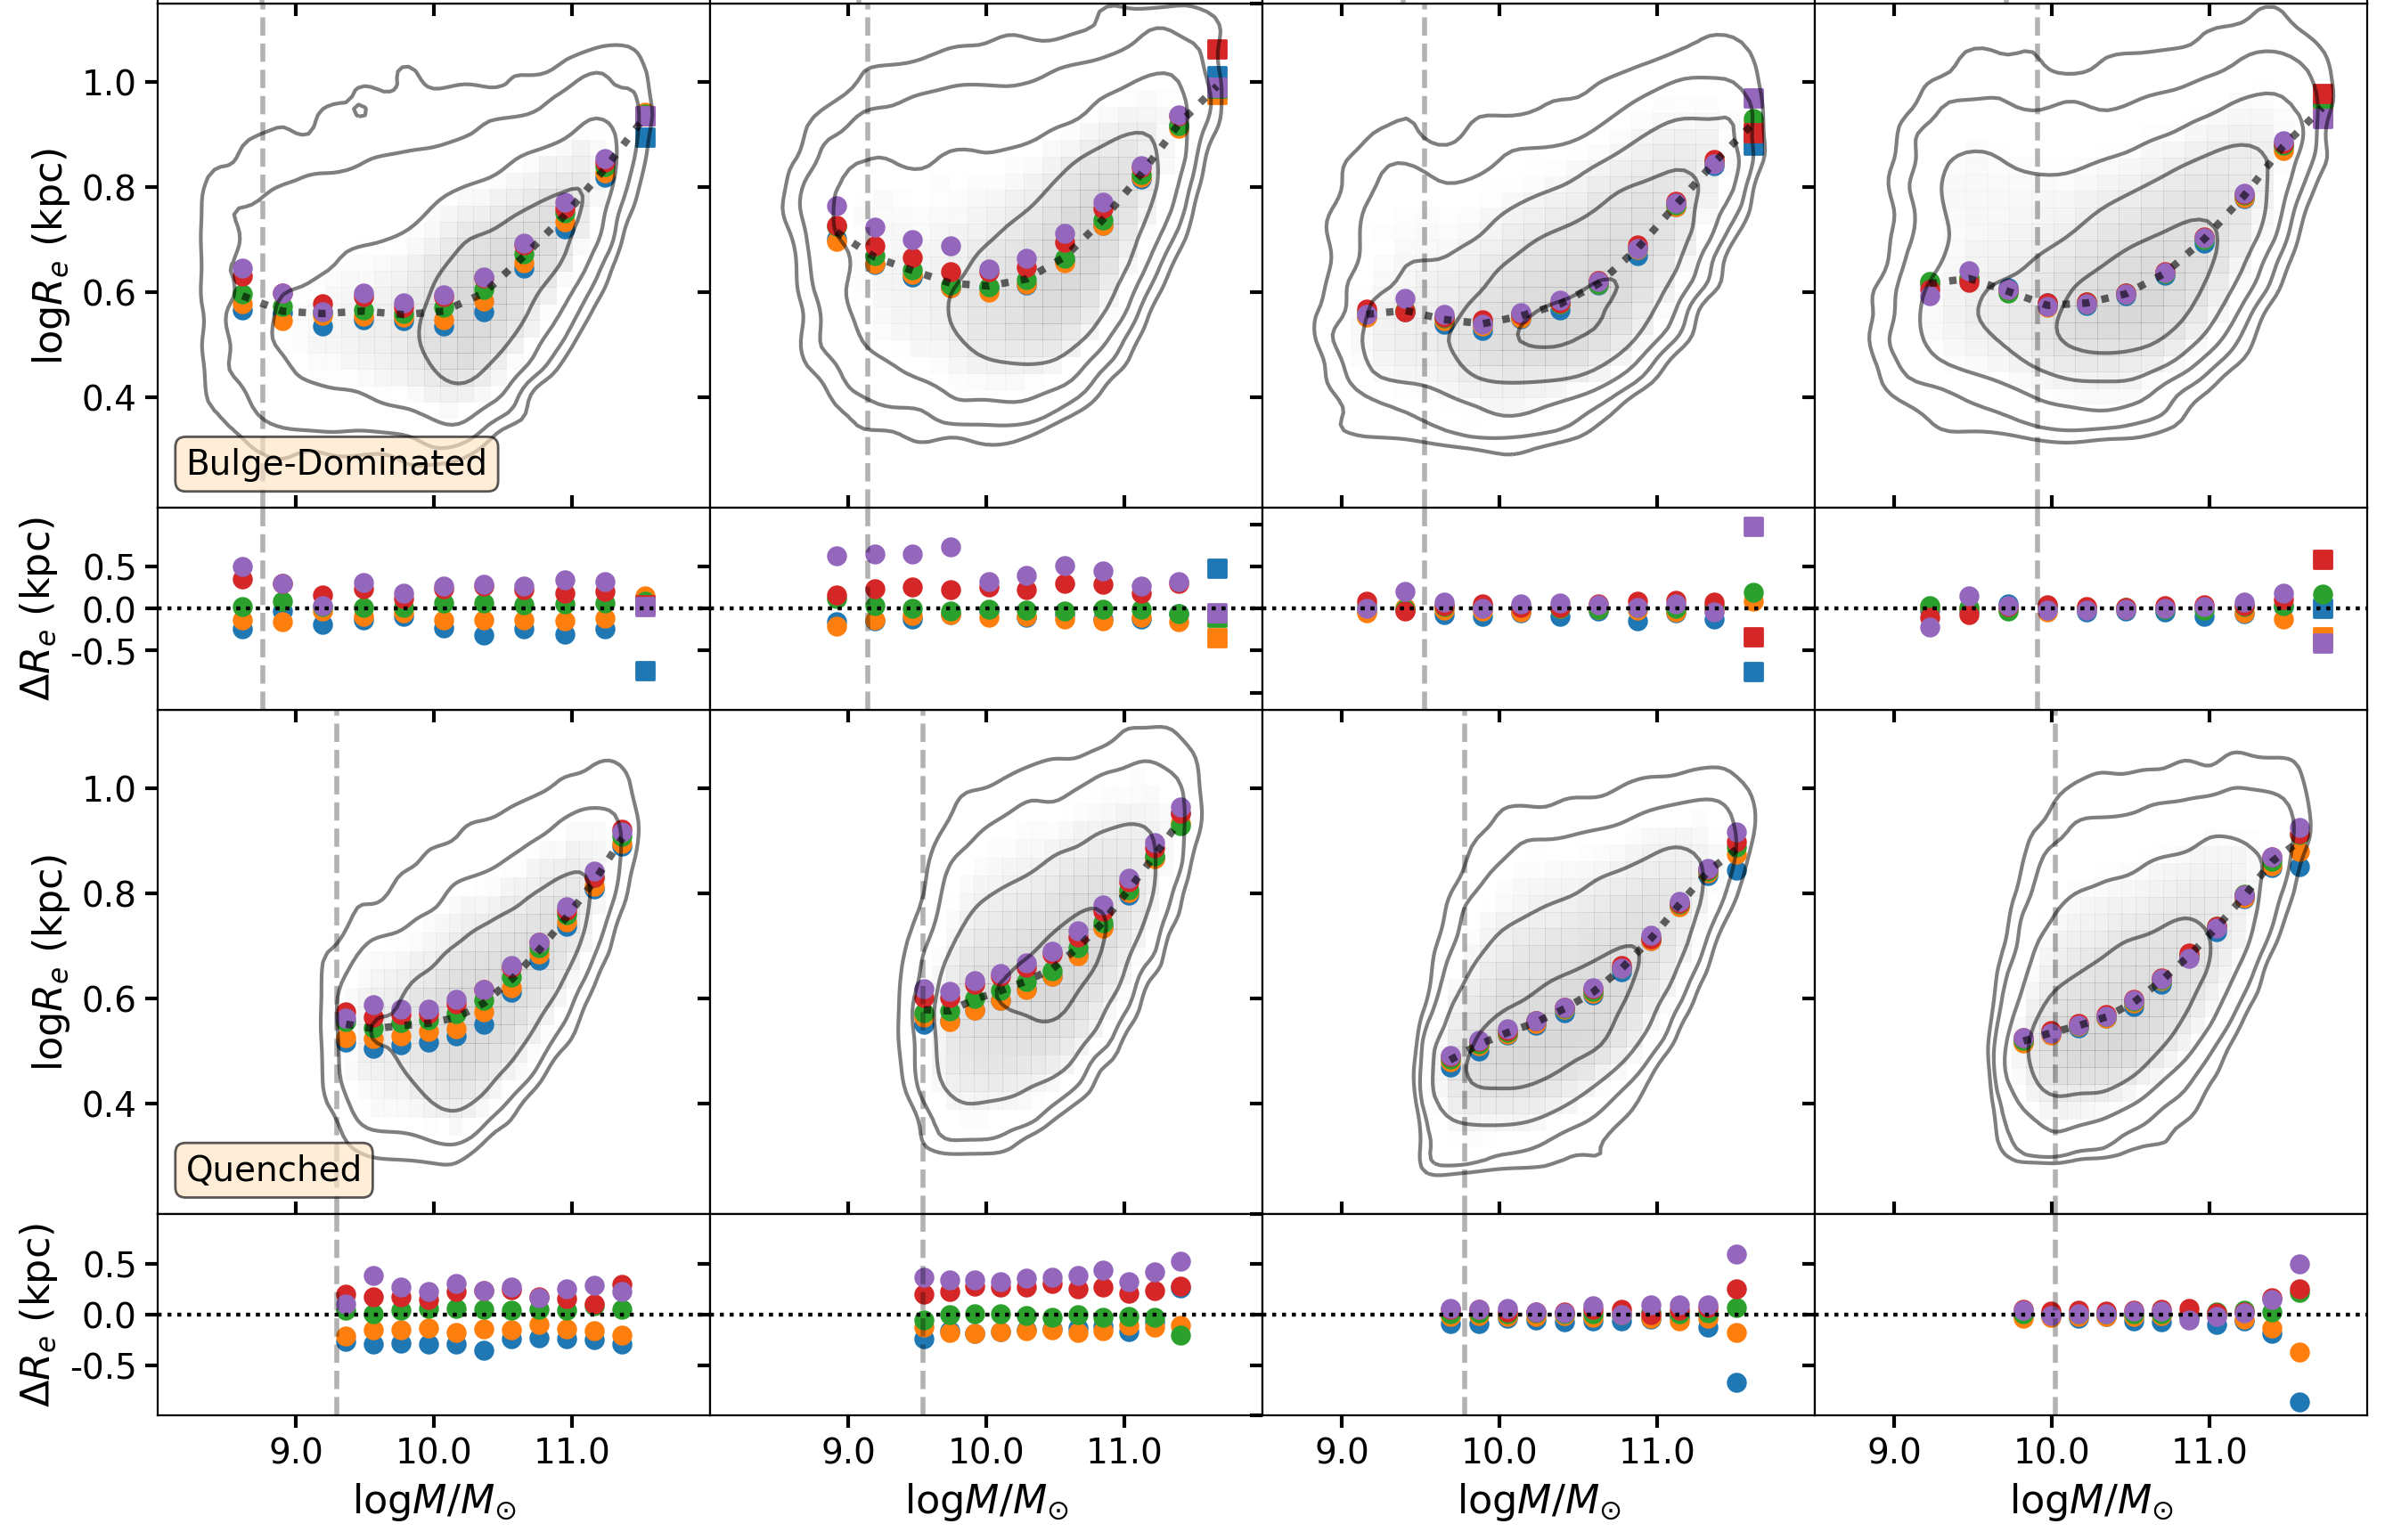
\includegraphics[width=0.95\textwidth]{r_m_sub_2.png}} 
  \end{center}
  \caption{The size-mass relationship is shown above (top panels) in the four different redshift slices (four columns) for different sub-populations of galaxies (four rows). The colored points in the top panels depict the median effective radius at a given stellar mass for all galaxies within a given density excess bin. The black dotted lines running alongside the colored points show the overall trend. The bottom panels, underneath each contour plot, show how the colored points deviate from the overall median trend line. The gray dashed vertical lines show the corresponding mass completeness limit in each redshift slice. Note that some of the colored points are squares (instead of circles) --- this indicates that there are less than 100 galaxies in these bins.}
    \label{fig_c4:r_m_sub}
\end{figure*}


In \S \ref{sec_c4:sep_into_subsamples}, we described how we split our total sample into sub-populations of disk-dominated, bulge-dominated, star-forming, and quiescent galaxies. In this section, we describe the results of running the same analysis we did in \S \ref{sec_c4:rad_den_all} for each sub-population. The $R_e$ v/s $\sigma_{r=10cMpc}$ plot for each sub-population is shown in Figure \ref{fig_c4:rad_den_sub}, and the results of the correlation analysis are reported in Table \ref{tab_c4:corr_subpop_ab}. To be concise, we only include order-of-magnitude values in Table \ref{tab_c4:corr_subpop_ab} and the interested reader can refer to Appendix \ref{sec_c4:ap:corr_coeff} for the unabridged version of this table. Finally, the size-mass diagram, plotted individually for each sub-population, is available in Figure \ref{fig_c4:r_m_sub}. The format of these figures and the table is similar to what was used in the last section for the overall analysis. 

As can be seen from Table \ref{tab_c4:corr_subpop_ab} and Figure \ref{fig_c4:rad_den_sub}, for $z < 0.5$, the positive correlation between $R_e$ and $\sigma_{r=10cMpc}$ can be confirmed with more than five sigma confidence for each individual sub-population. For disk-dominated and star-forming galaxies, the effect appears to be marginally stronger in the lower mass bin compared to the higher mass bin. On the other hand, for bulge-dominated and quiescent systems, the effect seems to be marginally stronger at the higher mass end compared to the lower mass end. 

In examining the two higher redshift slices, the effect is markedly lesser or entirely absent when contrasted with the lower redshift slices across each sub-population. However, for bulge-dominated and quiescent systems with $\log M/M_{\odot} > 10.25$, we can confirm the existence of a positive correlation. This correlation demonstrates a confidence level exceeding five sigma for both high redshift slices. At the lower mass end, the correlation is either non-existent or significantly diminished for these bulge-dominated/quiescent systems at higher redshifts.

For the higher mass $z \geq 0.5$ star-forming and disk-dominated systems, we also notice indications of a positive correlation. However, these observed correlations are noticeably less potent compared to the statistical significance we find in the bulge-dominated/quiescent systems. Occasionally, the significance of these correlations falls short of, or just barely meets the five sigma confidence threshold.

In line with expectations from previous studies \citep[e.g.,][]{mowla19, hsc_mass_size}, Figure \ref{fig_c4:r_m_sub} shows that the steeper slope of the size-mass relation at higher masses is primarily driven by bulge-dominated and quiescent systems. The change in the slope of the power law is significantly less prevalent for disk-dominated and star-forming galaxies. Even when broken down into sub-populations, we do not observe any dependence of the pivotal stellar mass on environmental density.

Figure \ref{fig_c4:r_m_sub} confirms the presence of the critical stellar mass of $\sim 10^{11.25}M_{\odot}$ for the $z \geq 0.5$ slices for each individual sub-population. However, we must note that because the sample was split into different groups, we can confirm this result at $>5\sigma$ confidence only for the disk-dominated and the quiescent systems using our correlation analysis. For the bulge-dominated and star-forming systems, this effect can only be confirmed at $\gtrapprox3\sigma$ confidence. It is also interesting to note that for galaxies above the critical mass, the $\Delta R_e$ is significantly higher for bulge-dominated and quiescent systems ($\sim1.2-1.5$ kpc) compared to disk-dominated and star-forming galaxies ($\sim0.6-0.8$ kpc). This is in line with the previous results in Table \ref{tab_c4:corr_subpop_ab} and Figure \ref{fig_c4:rad_den_sub}. 

\subsection{Variation of Morphology With Environment} \label{sec_c4:morph_env}
Having dealt with the variation of $R_e$ with environmental density, we now move to probe how the morphology of galaxies changes with environment. \gampen{} predicts the posterior distribution of $L_B/L_T$ for every galaxy, and we use the median value of the predicted distribution to split up the galaxies into disk-dominated ($L_B/L_T \leq 0.4$) and bulge-dominated ($L_B/L_T \geq 0.6$) sub-populations. We then study how these fractions vary as a function of $\sigma_{r=10cMpc}$.

\begin{figure*}[htb]
    \centering
    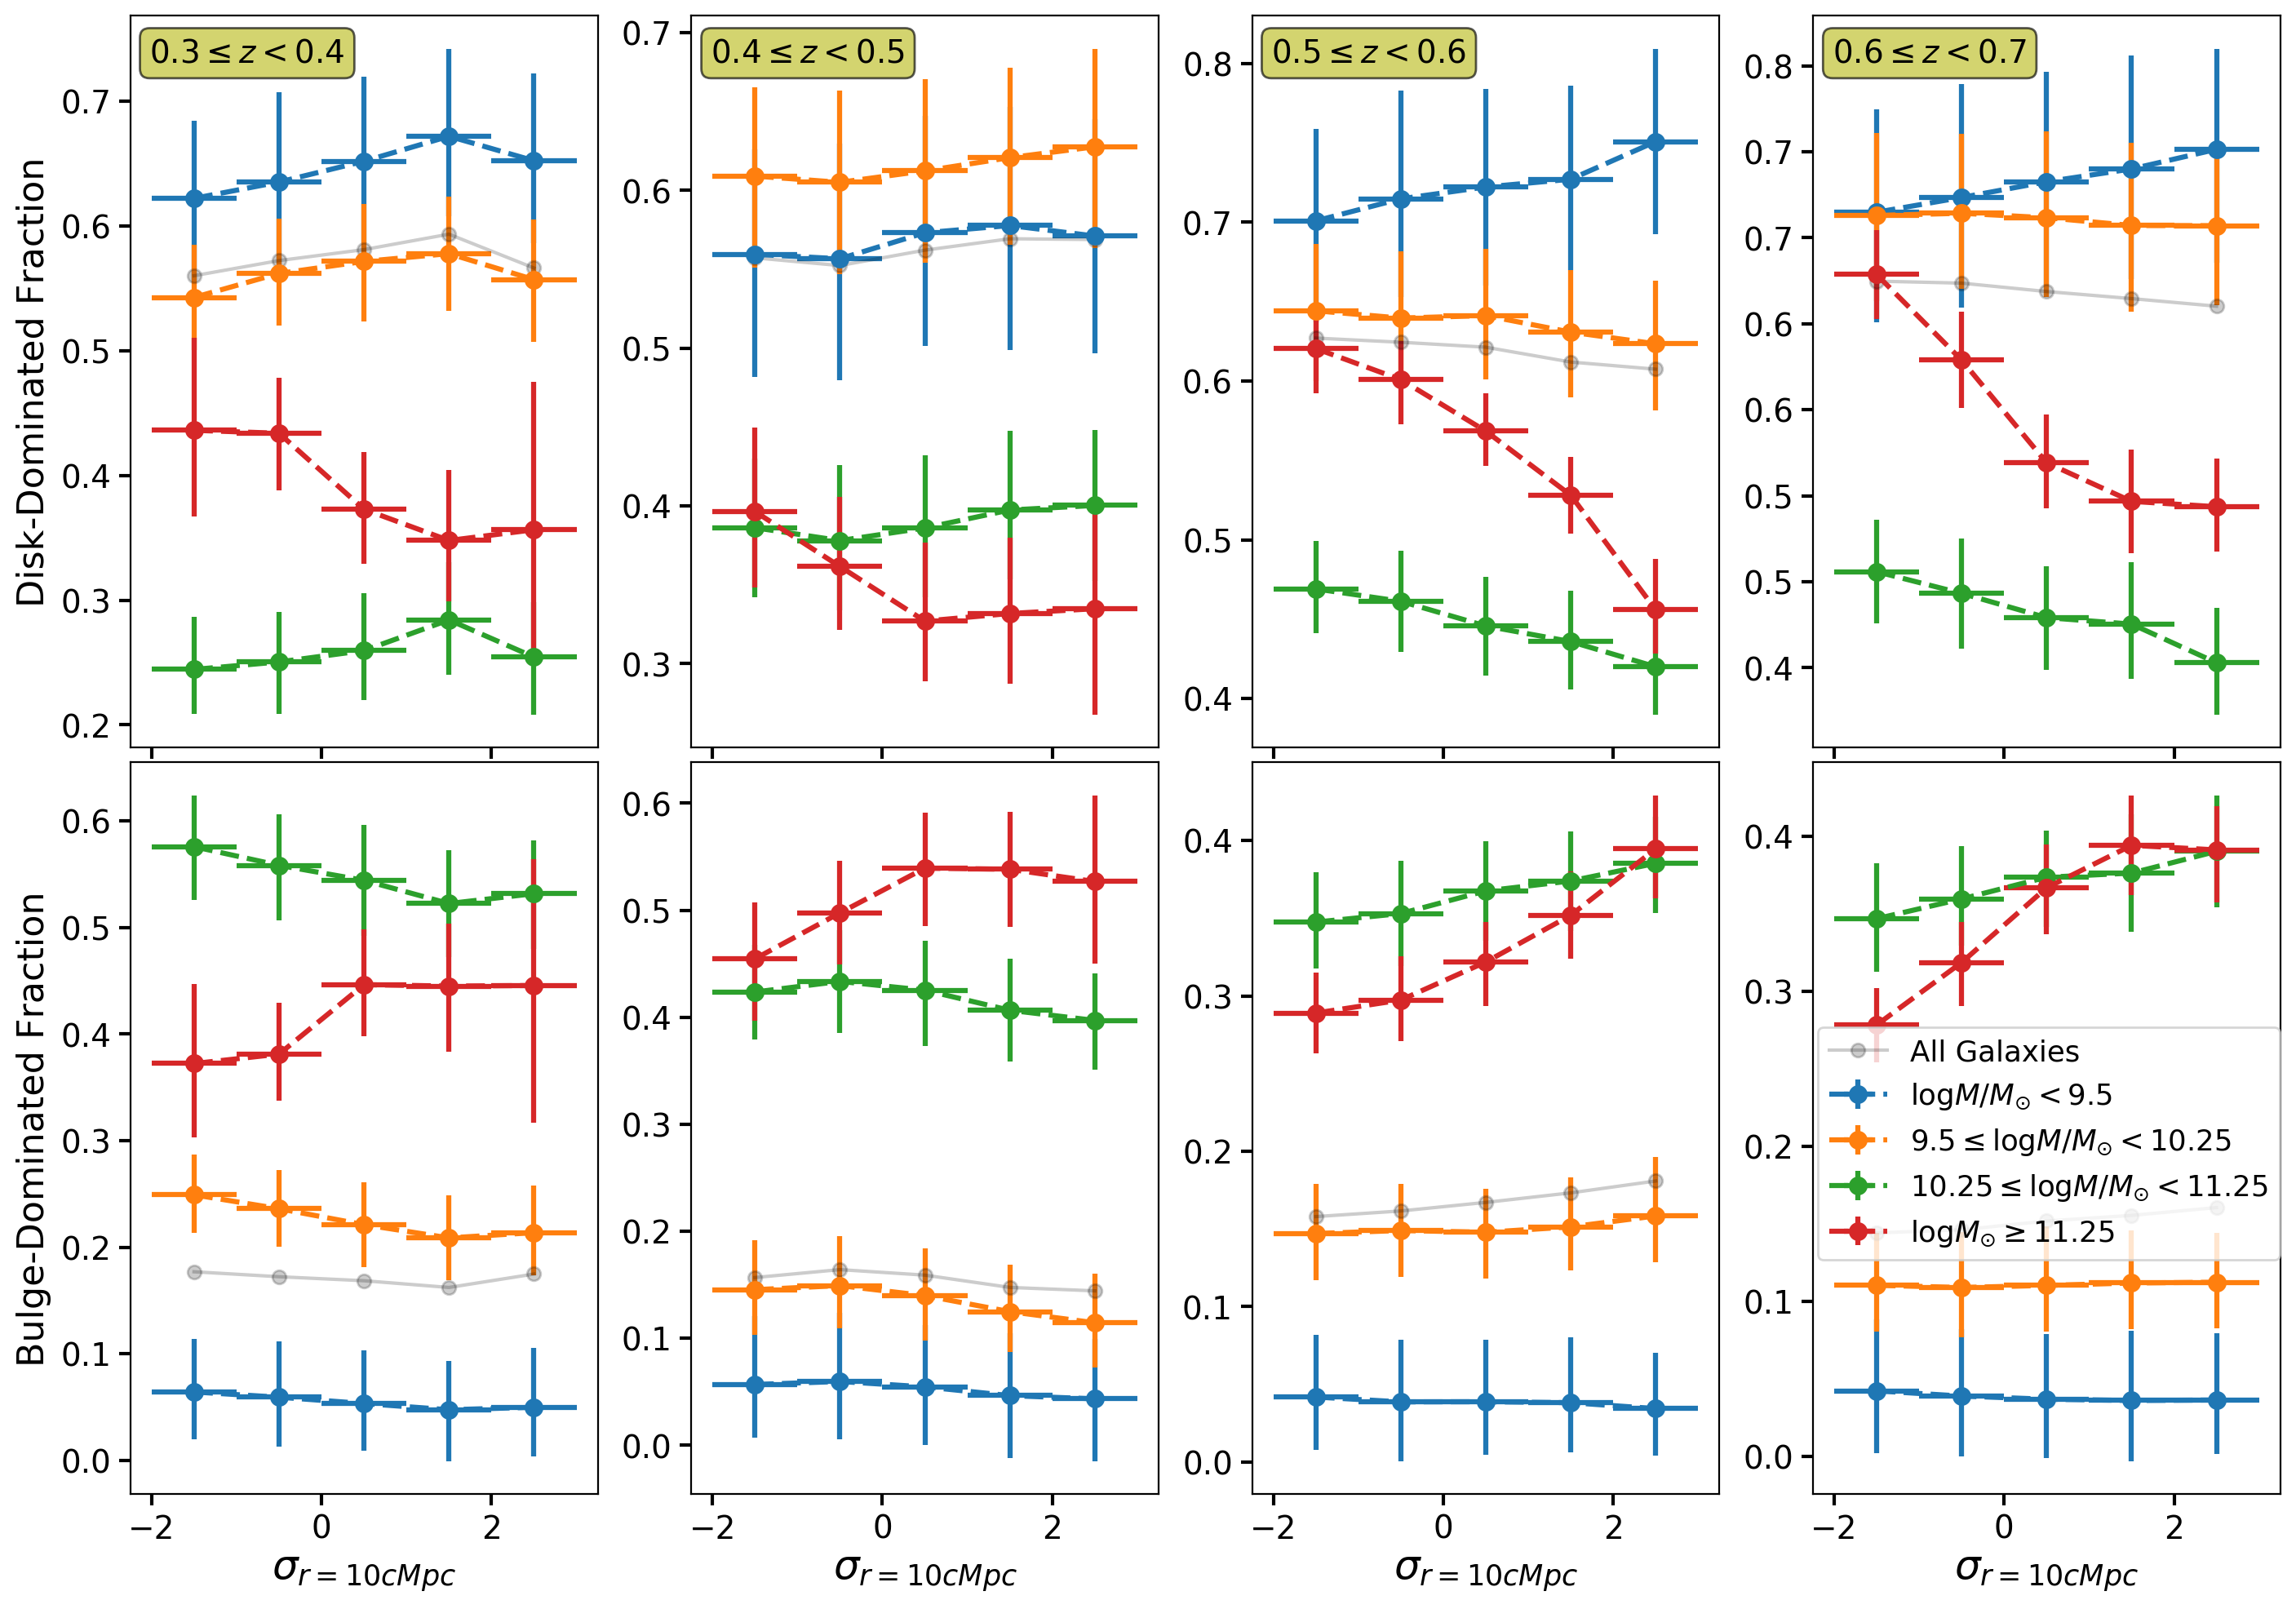
\includegraphics[width = \textwidth]{morph_den.png}
    \caption{The variation of morphological fractions with density excess is shown above, with each column depicting a different redshift slice. The colored lines represent different stellar mass ranges, as the figure legend denotes, with $M_c$ referring to the mass-completeness limit at the corresponding redshift. The top row shows the fraction of disk-dominated galaxies ($L_B/L_T \leq 0.4$) while the bottom row shows the fraction of bulge-dominated galaxies ($L_B/L_T \geq 0.6$). The points depict the fraction of galaxies with a given morphology with respect to all galaxies within the given stellar mass and density-excess bin. The vertical error bars represent the fractional uncertainties (i.e., $68\%$ confidence intervals) taking into account the uncertainties predicted by \gampen{} on $L_B/L_T$ measurements. The gray lines indicate the overall median trend.}
    \label{fig_c4:morph_den}
\end{figure*}

Figure \ref{fig_c4:morph_den} shows how the measured fractions vary for the four redshift slices. Compared to Figure \ref{fig_c4:rad_den_all}, we have added an additional mass bin at the higher mass end. To estimate the error bars shown in Figure \ref{fig_c4:morph_den}, we sampled values of $L_B/L_T$ 5000 times for each galaxy from the predicted posterior distribution. Thereafter, we measured the bulge- and disk-dominated fractions for each of these 5000 draws. The error bars shown in Figure \ref{fig_c4:morph_den} represent the $68\%$ confidence interval of the distribution of disk- and bulge-dominated fractions.

We want to note that, as described above, our morphological classifications are based on numerical estimates of $L_B/L_T$. Thus, the disk- and bulge-dominated fractions measured above are not expected to be identical to measurements of early-type, late-type, or spiral morphological fractions identified using visual inspection or machine learning frameworks. Therefore, the following results should be interpreted in their own right, and care should be taken while comparing our results to previous studies that employed qualitative classification schemes. 

We find that for the highest mass bin ($\log M/M_{\odot} > 11.25$), the fraction of bulge-dominated galaxies increases in denser environments. In tandem, the fraction of disk-dominated galaxies drops correspondingly. We observe this effect in all four redshift slices, although the result is marginally more statistically significant and stronger in the higher two redshift bins.

The second highest mass bin ($10.25 \leq \log M/M_{\odot} < 11.25$ ) also displays a similar, but weaker trend in the higher two redshift slices.  In all other mass bin and redshift slice combinations, we do not observe any statistically significant correlations. Note that compared to \S \ref{sec_c4:rad_den}, we have much poorer statistics and it is difficult to confirm weak correlations here. This is driven by the fact that for all results in \S \ref{sec_c4:rad_den}, we had millions of data points. In contrast, here, the measured fractions aggregate over many galaxies, resulting in only five data points per mass bin. 

Another interesting fact to note is the overall ratio of disk- and bulge-dominated galaxies. For $z\geq0.5$, there are always more disk-dominated galaxies than bulge-dominated galaxies, with the two fractions becoming roughly equal at the highest densities for the two higher mass bins. In contrast, for $z < 0.5$, the relative fractions appear to be completely dependent on mass. For $\log M/M_\odot < 10.25$, there are more disk-dominated galaxies than bulge-dominated galaxies. While for higher masses, the fraction of disk-dominated galaxies is roughly equal to or lesser than the number of bulge-dominated galaxies.  


\section{Summary \& Discussion} \label{sec_c4:discussion}

In this section, we summarize the main findings from \S \ref{sec_c4:results}, compare our results to previous studies, and reflect on possible explanations for the observed correlations. 

\subsection{Summary of Observed Correlations} \label{sec_c4:summary}

For $0.3 \leq z < 0.5$:-

\begin{itemize}
    \item We can confirm with $>5 \sigma$ confidence that galaxies in denser environments are larger than their counterparts with similar masses in less-dense environments. 
    \begin{itemize}
        \item The above result holds true for the entire mass range probed in this study. We cannot detect any significant monotonic change in the strength of the correlation with mass (see lower panels of Figure \ref{fig_c4:r_m_all}). 
        \item However, the effect does appear to be marginally stronger in the higher mass-bin (see $\alpha$ in Table \ref{tab_c4:corr_all}).
    \end{itemize}
    \item The $> 5\sigma$ positive correlation between $R_e$ and $\sigma_{r=10cMpc}$ also holds individually for disk-dominated, bulge-dominated, star-forming, and quiescent sub-populations drawn from our total sample. 
    \begin{itemize}
        \item The above result also holds true for the entire mass range probed in this study and we cannot detect any significant monotonic change in the strength of the correlation with mass (see lower panels of Figure \ref{fig_c4:r_m_sub}).
        \item However, the effect does appear to be marginally stronger in the lower mass bin for disk-dominated/star-forming galaxies; and in the higher mass bin for bulge-dominated/quiescent galaxies (see $\alpha$ in Table \ref{tab_c4:corr_subpop_ab}).
    \end{itemize}  
    \item For galaxies with $\log M/M_\odot > 11.25$, the bulge-dominated fraction of galaxies grows in denser environments at the expense of the fraction of disk-dominated galaxies. For lower masses, we observe no statistically significant trends when considering the errors in our fraction measurements.
\end{itemize}

For $0.5 \leq z < 0.7$:-
\begin{itemize}
    \item The overall positive trend between galaxy radius and large-scale structure density is much weaker/negligible compared to the lower redshifts. 
    \begin{itemize}
        \item For $0.6 \leq z < 0.7$, we cannot detect any statistically significant correlation, while for $0.5 \leq z < 0.6$, we detect a $>5\sigma$ positive correlation only in the higher mass bin.
        \item However, there appears to be a critical stellar mass ($\sim2\times10^{11} M_\odot$) above which there is a strong preference for galaxies in denser environments to be larger. Although at the tail end of the mass distribution, we have enough statistics to confirm this effect $>5\sigma$ confidence. 
    \end{itemize}
    \item When the sample is divided into disk-dominated, star-forming, bulge-dominated, and quiescent galaxies:- we correspondingly find that the overall positive correlation seen at lower z disappears/weakens when compared within each sub-population.
    \begin{itemize}
        \item However, for $\log M/M_{\odot} > 10.25$ bulge-dominated and quiescent galaxies, we can detect a positive correlation with $>5\sigma$ confidence for both the higher redshift slices. This effect weakens/disappears in the lower mass bin. 
        \item For $\log M/M_{\odot} > 10.25$ star-forming and disk-dominated galaxies, we can also see indications of a positive correlation; however, the observed correlation and its statistical significance is weaker compared to the bulge-dominated/quiescent galaxies mentioned above. Occasionally, the significance of these correlations falls short of, or just barely meets the five sigma confidence threshold.
        \item The existence of the previously mentioned critical stellar mass ($\sim2\times10^{11} M_\odot$) can be observed for each sub-population, above which we see a clear correlation of radius and environmental density. This observed correlation above the critical stellar mass is stronger for bulge-dominated and quiescent systems compared to disk-dominated and star-forming systems. 
    \end{itemize}
    \item For galaxies with $\log M/M_\odot > 11.25$,  the bulge-dominated fraction of galaxies grows in denser environments at the expense of disk-dominated galaxies. For lower masses, we observe only marginal or no trends when considering the errors in our fraction measurements.
\end{itemize}

\subsection{Comparison to Previous Studies of Radius \& Environment} \label{sec_c4:comp}

The correlations detailed in \S \ref{sec_c4:summary} help us to understand the contradictory results previously reported in the literature, as outlined in Table \ref{tab_c4:lit_survey}. Since a galaxy's radius is primarily determined by stellar mass, examining its secondary dependence on environment necessitates a large, uniform sample. Our findings emphasize that this substantial sample must be supplemented by a robust analytical framework capable of predicting and accounting for uncertainties when assessing the existence of correlations.

All the studies referenced in Table \ref{tab_c4:lit_survey} used sample sizes that are smaller by a factor of $\sim100-10,000$ compared to this work. Furthermore, none of the previously mentioned studies utilized an end-to-end Bayesian framework like \gampen{}, thus lacking a robust handle on the uncertainty in their $R_e$ measurement\footnote{as shown in Chapter \ref{chap:hsc_morph}, light profile fitting tools underestimate uncertainties by $15-60\%$}. Nor did these studies incorporate errors into their correlation analysis in a statistically robust manner.

Therefore, given the low values of the observed correlation coefficients and their dependence on redshift, stellar mass, morphology, and star formation; it is not surprising that prior studies documented a range of positive, negative, and no correlations, as shown in Table \ref{tab_c4:lit_survey}. These earlier works  were limited in their scope, providing an examination of a narrow segment of all galaxies rather than a comprehensive overview. In fact, if we restrict our total sample size to $\sim1000$ galaxies and repeat our analysis without taking into account $R_e$ errors, we cannot reproduce our own results with high statistical significance. Every time we draw a different sample from all the galaxies and the $R_e$ distribution of each galaxy, we observe markedly varying trends.

Some of the previous studies probing $z > 0.5$ have observed the correlation solely for passive / quiescent / early-type galaxies \citep[e.g.,][]{Cooper12,Lani13,Bassett13}. This agrees with the fact that in our study at $z > 0.5$, the statistical significance of the observed correlation is much stronger for higher mass quiescent and bulge-dominated galaxies. Additionally, \citet{Afonso19} observed the correlation only for galaxies with $\log M/M_{\odot} > 11$. This almost perfectly coincides with the critical stellar mass we observed for $z > 0.5$ galaxies. 

\subsection{Possible Explanations of Observed Correlations} \label{sec_c4:theory}
Given our current understanding of the hierarchical model of galaxy formation in the $\Lambda$ cold dark matter ($\Lambda$CDM) paradigm, galaxy sizes are affected by a host of different factors. Comprehensive follow up work using N-body and cosmological simulations is needed to definitively determine the cause of the correlations we observe. However, given the existing body of literature, it is possible to point to a few different reasons that could have led to the correlations that we observe in \S \ref{sec_c4:results}.

Classical models of galaxy formation \citep[e.g.,][]{fall80,mo98} based the radial sizes of galaxies on the spin of their dark matter halos and predicted that galaxy sizes should be proportional to the spin and size ($R_{vir}$) of the halo. Since then, there have been several follow-up studies using the standard abundance matching model in N-body simulations as well as using zoom-in cosmological simulations \citep[e.g.,][]{Kravtsov13, somerville18, jiang19}, all of which have converged on the general prediction

\begin{equation}
    R_e = A R_{vir}
    \label{eq_c4:r_e_vir}
\end{equation}

\noindent although the predicted nature of A has varied. Different studies have predicted A to be either constant or dependent on halo concentration and/or halo spin. We refer the interested reader to \citet{wechsler_tinker} for an extended discussion.

It is well known that in the $\Lambda$CDM paradigm, the clustering of dark matter halos depends on various halo properties in addition to halo mass \citep[e.g.,][]{wechsler02,wechsler06,gao07} -- this is commonly referred to as `assembly bias' (see \citet{mao18} for a recent overview). As a consequence of this effect, larger halos (of the same mass) typically reside in denser environments, and  halos (of the same mass) with higher concentration and spin are known to cluster more strongly. 

Therefore, it can be expected from Eq. \ref{eq_c4:r_e_vir} that galaxies in denser environments will be preferentially larger compared to equally massive counterparts in less-dense environments. Given that we observe the correlation between $R_e$ and $\sigma_{r=10cMpc}$ for each of the sub-populations, we posit that assembly bias might be the primary driving factor behind the overall correlations we observe in \S \ref{sec_c4:results} for the entire sample. The fact that Eq. \ref{eq_c4:r_e_vir} has been found to hold true for almost all morphological types and across a wide range of stellar masses \cite[e.g.,][]{Kravtsov13} could explain why we can observe the effect (at lower z) for all mass ranges and all sub-populations of galaxies. 

\citet{somerville18} found the ratio between stellar-radius and halo-radius ($A$ in Eq. \ref{eq_c4:r_e_vir}) to be only weakly dependant on mass and reported that $A$ increases by a factor of 1.5 from $z\sim3$ to $z\sim0.4$ for galaxies with $\log M/M_{\odot} \gtrapprox 10$. This is consistent with what we find:- overall, the strength of the correlation between $R_e$ and $\sigma_{r=10cMpc}$ is weakly dependent on stellar mass and is stronger at lower redshifts. 

The fact that we observe a stronger correlation for massive bulge-dominated and quiescent systems at $z > 0.5$ can be understood from the perspective of the correlation between size growth in these systems and mergers. It has been proposed by many that for bulge-dominated/quiescent systems, size-growth at higher masses is dominated by minor, dry mergers \citep[e.g.,][]{shankar13} and the same conclusion has also been drawn from observational results \citep[e.g.,][]{mowla19,hsc_mass_size}. Given that mergers are more efficient and frequent in denser environments, bulge-dominated/quiescent systems in dense environments undergo a more rapid size evolution compared to their equally massive counterparts in lower-density environments --- resulting in larger quiescent galaxies in denser environments. The fact that the increased correlation for bulge-dominated/quiescent systems is mostly observed in the higher redshift slices could be due to the fact that mergers are thought to be more prevalent at higher redshifts. Since size growth at lower masses and for disk-dominated/star-forming systems is not dominated by mergers, it is not surprising that the observed correlations are weaker for these cases. 


Mergers could also explain the existence of the critical stellar mass observed at $z \geq 0.5$. $\log M/M_{\odot} \sim 11.25$ may represent a critical stellar mass beyond which mergers play an increased role in the size and mass growth of both disk-dominated/star-forming and bulge-dominated/quiescent systems at $z \geq 0.5$. Given that mergers are more prevalent and efficient in denser environments, this would explain why we always see a strong correlation between $R_e$ and $\sigma_{r=10cMpc}$ for galaxies with $\log M/M_{\odot} \geq 11.25$.

%Mergers could also play a partial role in explaining the overall redshift evolution of the observed correlations. As time progresses, galaxies become more gas-poor, and thus, galaxies closer to the present epoch are thought to have been preferentially born from a series of gas-poor mergers. Given that mergers are more prevalent and efficient in denser environments, this could partly explain why we see a stronger correlation at lower redshifts.

The trend we observe between galaxy morphology and environmental density in Figure \ref{fig_c4:morph_den} is largely consistent with what has been reported previously. The results indicate that the transformation of (star-forming) disk-dominated galaxies into (quiescent) bulge-dominated galaxies occur at an accelerated rate in denser environments. Given that various effects responsible for such a transformation (e.g., mergers, ram pressure stripping, gas strangulation) are more prevalent in denser environments, it is not surprising that we observe the rate of morphological transformation to be more in denser regions. The fact that we do not observe this correlation at lower masses can be due to two reasons:- i) massive galaxies are more likely to experience mergers compared to less massive galaxies; ii) bulge/disk decomposition is more challenging for smaller, less-massive galaxies, which leads to higher uncertainties in $L_B/L_T$ measurements. 

\section{Conclusions} \label{sec_c4:conclusions}

In this work, we presented one of the first comprehensive studies of the variation of galaxy radius with environment beyond $z \geq 0.2$. We used a comprehensive sample of $\sim3$ million HSC galaxies in the redshift range $0.3 \leq z < 0.7$ with masses down to $\log M/M_{\odot}\sim8.9$. This represents a $\sim100-10,000$ times increase in sample size and a $\sim1$ dex improvement in mass completeness compared to most previous studies. We combined this extensive sample with robust estimates of structural parameters and associated uncertainties from \gampen{}, allowing us to perform a statistically robust correlation analysis using Monte-Carlo sampling.  Using the above sample, we also revisited the correlation between morphology and environment. The following are the primary takeaways:- 

\begin{itemize}
    \item We confirm with $>5\sigma$ confidence that galaxy radius is positively correlated with environment, even when controlling for stellar mass. At the scales considered in this study (10 co-moving Mpc), galaxies in denser environments are consistently $\sim10-20\%$ larger than equally massive galaxies in less dense environments. 
    \item We find that the strength of the above correlation is dependent on redshift, stellar mass, and galaxy morphology. The correlation is strongest at $z < 0.5$ and becomes systematically weaker/disappears at $z \geq 0.5$.
    \item At $z < 0.5$, we find the overall correlation to be persistent (at $>5\sigma$ confidence) across the entire stellar mass range covered in this study and individually across all sub-populations -- disk-dominated, bulge-dominated, star-forming, and quiescent galaxies. For disk-dominated/star-forming galaxies, the correlation is marginally stronger at lower masses; while for bulge-dominated/quiescent galaxies, it is marginally stronger at higher masses. 
    \item At $z\geq0.5$, although the overall correlation is weaker/absent, some noteworthy deviations exist. For bulge-dominated and quiescent systems with $\log M/M_{\odot} > 10.25$, we observe a strong $>5\sigma$ correlation. We also find the existence of a critical stellar mass ($\log M/M_{\odot} \sim 11.25 \sim 2\times 10^{11}$), beyond which there is a strong correlation present in the overall sample. The critical stellar mass is also observed to be present individually for all studied sub-populations of galaxies. 
    \item Consistent with previous results, we find that (when controlling for stellar mass) the fraction of bulge-dominated galaxies grows in denser environments at the expense of disk-dominated galaxies. We find the relationship to be strongest at the highest stellar masses, with lower mass ranges displaying weak/no statistically significant correlation.
\end{itemize}

We posit that assembly bias in dark matter halos could be the principal driving factor behind the observed correlations between radius and environment in the overall sample. Due to assembly bias, larger halos (of the same mass) typically reside in denser environments, and  halos (of the same mass) with higher concentration and spin cluster more strongly. Additionally, galaxy formation models have predicted that galaxy sizes should be correlated with the size/spin/concentration of their dark matter halos or combinations thereof. This would therefore result in larger galaxies preferentially residing in denser environments. The above theoretical framework provides a consistent explanation for most of the correlations outlined above.

The observed stronger correlation for massive bulge-dominated/quiescent systems and the existence of the critical stellar mass at $z > 0.5$ may be driven by mergers. We posit that minor, dry mergers dominate size growth in these systems. Given that mergers are more efficient and frequent in denser environments, the above-mentioned sub-populations undergo a more rapid size evolution compared to their equally massive counterparts in lower-density environments.

The trend we observe between galaxy morphology and environmental density is driven by disk-dominated galaxies being transformed into bulge-dominated galaxies at an accelerated rate in denser environments. This is not surprising given that various effects responsible for such a transformation (e.g., mergers, ram pressure stripping, gas strangulation) are more prevalent in denser environments. 

This comprehensive study represents an important first step in resolving decades of contradictory results on the correlation between galaxy size and environmental density. Our findings emphasize that earlier works were limited in their scope, examining a narrow segment of all galaxies rather than a comprehensive overview. These previous conflicting results were largely driven by the use of small non-uniform samples and the failure to properly account for measurement uncertainties while assessing the presence of correlations. 

Comparative theoretical follow-up work using N-body and cosmological simulations is needed to expand on the theoretical framework we presented above and conclusively establish the reason for the observed correlations. Such future efforts will also be greatly assisted by current/upcoming large spectroscopic programs such as the Dark Energy Spectroscopic Instrument \citep[DESI;][]{desi} and the Subaru Prime Focus Spectrograph \citep[PFS;][]{pfs}. These spectroscopic surveys will empower us to investigate the correlation between structural parameters and environment over a comparable volume at much finer scales. They will eliminate the need to use redshift slices and enable the use of angular correlation functions. Finally, upcoming space-based wide-field surveys such as Euclid \citep{euclid} and the Nancy Grace Roman Space Telescope \citep[NGRST;][]{ngrst} will allow us to perform similar comprehensive analyses at higher redshifts. 


\section*{Chapter Acknowledgments}
C.M.U. and A.G. would like to acknowledge support from the National Aeronautics and Space Administration via ADAP Grant 80NSSC18K0418. 

A.G. would like to acknowledge the support received from the Yale Graduate School of Arts \& Sciences through the Dean's Emerging Scholars Research Award.

A.G. would like to acknowledge helpful discussions with Kaustav Mitra. 

The Hyper Suprime-Cam (HSC) collaboration includes the astronomical communities of Japan and Taiwan, and Princeton University. The HSC instrumentation and software were developed by the National Astronomical Observatory of Japan (NAOJ), the Kavli Institute for the Physics and Mathematics of the Universe (Kavli IPMU), the University of Tokyo, the High Energy Accelerator Research Organization (KEK), the Academia Sinica Institute for Astronomy and Astrophysics in Taiwan (ASIAA), and Princeton University. Funding was contributed by the FIRST program from Japanese Cabinet Office, the Ministry of Education, Culture, Sports, Science and Technology (MEXT), the Japan Society for the Promotion of Science (JSPS), Japan Science and Technology Agency (JST), the Toray Science Foundation, NAOJ, Kavli IPMU, KEK, ASIAA, and Princeton University. 

This paper makes use of software developed for the Large Synoptic Survey Telescope. We thank the LSST Project for making their code available as free software at  \href{http://dm.lsst.org}{http://dm.lsst.org}.

The Pan-STARRS1 Surveys (PS1) have been made possible through contributions of the Institute for Astronomy, the University of Hawaii, the Pan-STARRS Project Office, the Max-Planck Society and its participating institutes, the Max Planck Institute for Astronomy, Heidelberg and the Max Planck Institute for Extraterrestrial Physics, Garching, The Johns Hopkins University, Durham University, the University of Edinburgh, Queen’s University Belfast, the Harvard-Smithsonian Center for Astrophysics, the Las Cumbres Observatory Global Telescope Network Incorporated, the National Central University of Taiwan, the Space Telescope Science Institute, the National Aeronautics and Space Administration under Grant No. NNX08AR22G issued through the Planetary Science Division of the NASA Science Mission Directorate, the National Science Foundation under Grant No. AST-1238877, the University of Maryland, and Eotvos Lorand University (ELTE) and the Los Alamos National Laboratory.

Based, in part, on data collected at the Subaru Telescope and retrieved from the HSC data archive system, which is operated by Subaru Telescope and Astronomy Data Center at National Astronomical Observatory of Japan.




